\documentclass[12pt,a4paper,twoside]{report}
\usepackage[italian]{babel}
\usepackage{newlfont}
\usepackage{color}
\textwidth=450pt\oddsidemargin=0pt

% INIZIO HEADER INSERITI DA ME, DA CUI HO TOLTO GLI HEADER CHE SI RIPETONO

%\documentclass[12pt,a4paper]{article}
%\usepackage[utf8]{inputenc}
\usepackage{titling}
\usepackage[backend=bibtex,
			style=numeric,
			sorting=none
			]{biblatex}
\addbibresource{bibliography.bib} %Import the bibliography file
%\setlength{\droptitle}{-2cm}% change title position
\usepackage{amsmath}
%\usepackage{amsfonts}
\usepackage{amssymb}
%\usepackage[T1]{fontenc}
\usepackage{tablefootnote}
\usepackage{multirow}
\usepackage{array}
\newcolumntype{P}[1]{>{\centering\arraybackslash}p{#1}}
\newcolumntype{M}[1]{>{\centering\arraybackslash}m{#1}}
\usepackage{graphicx}
\graphicspath{{images/}}
\usepackage[version=4]{mhchem}
%\usepackage{siunitx}
\usepackage{float}
\usepackage[top=1.7in,left=1in,right=1in]{geometry}
%\usepackage{listings}
%\usepackage{circuitikz}
\usepackage{tikz-feynman}
\usepackage{subcaption}
\usepackage{tabularx}
%\renewcommand{\lstlistingname}{Code}
%\renewcommand{\lstlistlistingname}{List of Code}
%\lstdefinestyle{chstyle}{
	%	backgroundcolor=\color{gray!12},
	%	basicstyle=\ttfamily\small,
	%	commentstyle=\color{green!60!black},
	%	keywordstyle=\color{magenta},
	%	stringstyle=\color{blue!50!red},
	%	showstringspaces=false,
	%	%captionpos=b,
	%	numbers=left,
	%	numberstyle=\footnotesize\color{gray},
	%	numbersep=10pt,
	%	%stepnumber=2,
	%	tabsize=2,
	%	frame=L,
	%	framerule=1pt,
	%	rulecolor=\color{red},
	%	breaklines=true,
	%	inputpath=code
	%}
%\renewmenumacro{\directory}{pathswithfolder} % default: path
%\renewmenumacro{\keys}{shadowedroundedkeys} % default: roundedkeys
\setlength{\arrayrulewidth}{0.9pt}
\renewcommand{\arraystretch}{1.3}
\usepackage{mathcomp}

%\usepackage{fontspec}
%\setmainfont{Calibri}

\usepackage{fancyhdr}
\pagestyle{fancy}
%\renewcommand{\chaptermark}[1]{\markboth{\MakeUppercase{\chaptername\ \thechapter.\ #1}}{}}
\renewcommand{\chaptermark}[1]{\markboth{\MakeUppercase{CAP.\ \thechapter\ --\ #1}}{}}
\setlength{\headwidth}{15cm} % la larghezza delle tabelle è di 1 cm inferiore (14cm)
\fancyhead{} % clear all header fields
\fancyhead[LO]{\footnotesize \textsl{\rightmark}}
\fancyhead[RE]{\footnotesize \textsl{\leftmark}}
\fancyhead[LE,RO]{\footnotesize \thepage}
\fancyfoot{} % clear all footer fields
\renewcommand{\headrulewidth}{0.3pt}

% è già di default interlinea singola
\usepackage{setspace}

\newsavebox{\largestimage}

%\usepackage[font=it]{caption}
%\usepackage{indentfirst}
%\interfootnotelinepenalty=\@M

\usepackage{hyperref}
\hypersetup{
	colorlinks,
	citecolor=black,
	filecolor=black,
	linkcolor=black,
	urlcolor=black
}

% FINE HEADER INSERITI DA ME

\begin{document}
	\pagenumbering{roman}
	\begin{titlepage}
		\begin{center}
			{{\Large{\textsc{Alma Mater Studiorum $\cdot$ Universit\`a di Bologna}}}} 
			\rule[0.1cm]{15.8cm}{0.1mm}
			\rule[0.5cm]{15.8cm}{0.6mm}
			\\\vspace{3mm}
			
			{\small{\bf Scuola di Scienze \\ 
					Dipartimento di Fisica e Astronomia\\
					Corso di Laurea in Fisica}}
			
		\end{center}
		
		\vspace{23mm}
		
		\begin{center}\textcolor{red}{
				%
				% INSERIRE IL TITOLO DELLA TESI
				%
				{\LARGE{\bf TITOLO TESI}}\\
		}\end{center}
		
		\vspace{50mm} \par \noindent
		
		\begin{minipage}[t]{0.47\textwidth}
			%
			% INSERIRE IL NOME DEL RELATORE CON IL RELATIVO TITOLO DI DOTTORE O PROFESSORE
			%
			{\large{\bf Relatore: \vspace{2mm}\\\textcolor{red}{
						Prof./Dott. Nome Cognome}\\\\
					%
					% INSERIRE IL NOME DEL CORRELATORE CON IL RELATIVO TITOLO DI DOTTORE O PROFESSORE
					%
					% SE NON AVETE UN CORRELATORE CANCELLATE LE PROSSIME 3 RIGHE
					%
					\textcolor{red}{
						\bf Correlatore: (eventuale)
						\vspace{2mm}\\
						Prof./Dott. Nome Cognome\\\\}}}
		\end{minipage}
		%
		\hfill
		%
		\begin{minipage}[t]{0.47\textwidth}\raggedleft {
				{\large{\bf Presentata da:
						\vspace{2mm}\\
						Simone Pasquini}}}
		\end{minipage}
		
		\vspace{40mm}
		
		\begin{center}
			Anno Accademico { 2023/2024}
		\end{center}
		
	\end{titlepage}
	\newpage
	\newgeometry{top=4cm,bottom=4cm,left=3cm,right=3cm}
	\onehalfspacing % Also singlespacing, doublespacing 
	\chapter*{Sommario (TBD)}
		Questo è l'inizio del sommario.
	\newpage
	\tableofcontents
	\newpage
	\addcontentsline{toc}{chapter}{Introduzione (TBD)}
	\chapter*{Introduzione (TBD)}
		Questo è l'inizio dell'introduzione. metodo del SSN (sistema già attivo nella sanità+Questo percorso ha portato alla marcatura CE del centro e nel 2017 l'adroterapia è stata inserita nei Livelli Essenziali di Assistenza.
		
		 statale).https://scienzapertutti.infn.it/4-adroterapia-dalla-fisica-alla-terapia
	\newpage
	
	\pagenumbering{arabic}
	
	\chapter{Terapie oncologiche e radiazioni ionizzanti}
	\section{Incidenza tumorale nel mondo}\label{sec:1.1}
	Tra le principali cause di morte della popolazione mondiale è possibile annoverare le neoplasie (o tumori) ovvero neoformazioni che, a causa di mutazioni genetiche che sfuggono ai meccanismi di controllo della proliferazione cellulare, iniziano a crescere, senza alcuna finalità, in maniera incontrollata e scoordinata rispetto al tessuto sano. \`E possibile distinguere due tipi di neoplasie: benigne e maligne. Mentre le prime si limitano alla sede di origine, le seconde generano metastasi, un processo in cui le cellule neoplastiche si spostano dalla sede originaria e danno origine a masse anomale che invadono altri tessuti dell'organismo, ostacolandone le funzioni vitali. In questo ultimo caso si parla di tumore maligno o cancro.
	
	Attualmente, è possibile prevenire fino al $50\%$ di tumori evitando fattori di rischio e implementando strategie di prevenzione già esistenti (cita
	%https://www.who.int/news-room/fact-sheets/detail/c+ancer
	), anche se ciò dipende dalla tempestività delle diagnosi, dalla tipologia delle cure e dal tipo di tumore. Si stima che nei Paesi industrializzati,\footnote{Si fa riferimento ai Paesi OCSE (Organizzazione per la Cooperazione e lo Sviluppo Economico).} nel $2021$, il cancro è la seconda causa di morte (causando il $21\%$ dei decessi totali), preceduto dalle malattie cardiovascolari (cita %https://www.oecd-ilibrary.org/docserver/7a7afb35-en.pdf?expires=1709230714&id=id&accname=guest&checksum=FBEABF3EDA6F2040465BB27356B8D68B
	). Sebbene il tasso di mortalità sia sceso sin dal $2000$, a livello mondiale il numero di casi diagnosticati di cancro (nel $2022$) attesta a quasi $20.0$ milioni\footnote{Negli ultimi dieci anni il numero di casi di tumore è aumentato di anno in anno, soprattutto a causa dell'invecchiamento progressivo della popolazione (cita
	%https://www.iss.it/-/tumori-in-aumento-le-diagnosi-in-europa-anche-per-effetto-dell-invecchiamento-demografico
	), ma nel biennio $2020$-$2021$ il trend è cambiato a causa della pandemia di COVID-$19$, che ha precluso l'accesso a screening oncologici (nel periodo gennaio--ottobre $2020$ vi è stato un calo del $37.3\%$ di test diagnostici rispetto al periodo pre-pandemico) (cita
	%https://www.ncbi.nlm.nih.gov/pmc/articles/PMC9807424/
	). Ciò potrebbe rivelarsi fatale nel medio-lungo termine causando un aumento dei tassi di incidenza e mortalità (cita
	%https://doi.org/10.1787/ae3016b9-en
	).} (pari al $2.5\tcperthousand$ della popolazione totale (citare %https://data.unicef.org/resources/data_explorer/unicef_f/?ag=UNICEF&df=GLOBAL_DATAFLOW&ver=1.0&dq=WORLD.DM_POP_TOT.&startPeriod=2022&endPeriod=2022
	)), di cui il $48.8\%$ hanno portato alla morte del paziente (citare
	%https://gco.iarc.who.int/en
	). Inoltre, i tassi di mortalità dovuti alle patologie tumorali sono strettamente dipendenti dall'indice di sviluppo dei Paesi (ISU), infatti da un tasso di mortalità del $39.2\%$ dei Paesi con ISU molto alto, si sale sino al $67.1\%$ dei Paesi con basso ISU (cita
	%https://gco.iarc.who.int/today/en/dataviz/bars?mode=population&key=total&group_populations=0&types=0_1&sort_by=value1&populations=900_981_982_983_984&multiple_populations=1&values_position=out&cancers_h=39&include_nmsc=1&age_end=17
	).
	
	Altri fattori rendono i tassi di incidenza e mortalità per patologie tumorali ulteriormente disuniformi, quali il sesso e l'età. A livello globale, l'incidenza di cancro negli uomini è più alta rispetto a quella delle donne dell'$8.0\%$ (cita
	%https://gco.iarc.who.int/media/globocan/factsheets/cancers/39-all-cancers-fact-sheet.pdf
	), dovuta anche al fatto che i primi si espongono maggiormente a fattori di rischio quali fumo e consumo di alcol. Inoltre, il $58\%$ di tumori viene diagnosticato nelle persone con più di 65 anni (cita
	%https://www.cdc.gov/cancer/uscs/about/data-briefs/no29-USCS-highlights-2019-incidence.htm
	).
	
	Sebbene i dati sopra citati testimonino la gravità delle patologie oncologiche, è indubbio che il progresso della scienza degli ultimi anni abbia permesso un notevole sviluppo nell'efficacia dei trattamenti oncologici: nel decennio $2010$--$2020$, il numero di persone che sopravvive dopo una diagnosi di cancro aumenta approssimativamente del $3\%$ in Paesi come l'Italia, gli Stati Uniti d'America, il Regno Unito e la Svizzera (cita
	%https://www.ncbi.nlm.nih.gov/pmc/articles/PMC5807846/pdf/12885_2018_Article_4053.pdf
	).
	
	\section{Terapie oncologiche}\label{sec:1.2}
	Il trattamento di un tumore avviene in molti modi differenti e varia in base al tipo di cancro, il suo stadio di avanzamento e dagli obiettivi che si intendono raggiungere al termine dei trattamenti. Oggigiorno, le terapie oncologiche si distinguono in locali (o regionali) e generali (o sistemiche), in base all'estensione del tumore che colpisce il paziente. Al primo gruppo appartengono terapie come la chirurgia, la radioterapia e l'adroterapia, mentre al secondo afferiscono la chemioterapia e l'immunoterapia. Tali tecniche, proprio per la loro diversità, sono spesso utilizzate in maniera complementare per aumentare l'efficacia dei trattamenti clinici. Per pianificare il trattamento più adeguato al fronte di una certa patologia oncologica, si introduce il concetto di stadiazione, che è un modo di descrivere in maniera schematica, rigorosa e standardizzata la grandezza di un tumore e la sua diffusione al di fuori della sede originale (cita
	%https://www.airc.it/cancro/affronta-la-malattia/la-fase-della-diagnosi/stadiazione
	). Le informazioni tipiche della stadiazione includono la collocazione del tumore, la sua estensione e se si è diffuso in parti del corpo differenti. Infatti, come già accennato, le cellule tumorali si moltiplicano in modo incontrollato andando a occupare (per mezzo del sistema linfatico o sanguigno) organi e tessuti distanti dalla sede di sviluppo originaria, attraverso un fenomeno chiamato metastatizzazione. Chiaramente, ciascuna terapia possiede effetti collaterali correlati all'azione distruttiva che si impiega per debellare la malattia oncologica.
	
	Se il tumore ha raggiunto un'estensione tale da formare metastasi, si scelgono trattamenti sistemici in modo che si possa debellare o, quantomeno, contenere la malattia oncologica. La chemioterapia consiste nella somministrazione di uno o più farmaci citotossici (o antiblastici) capaci di aggredire le cellule cancerose (cita
	%https://www.aimac.it/libretti-tumore/chemioterapia/che-cos-e-la-chemioterapia
	), mentre nell'immunoterapia si tenta di istruire il sistema immunitario affinché riconosca ed elimini le cellule malate che, in assenza di trattamento clinico, appaiono "nascoste" al sistema immunitario stesso.
	
	Qualora il tumore fosse localizzato, ben raggiungibile dall'esterno e sufficientemente lontano da organi vitali, si ricorre a operazioni chirurgiche, con le quali si asporta la massa tumorale dal corpo del paziente. Prima o dopo l'operazione chirurgica, si procede con tecniche radioterapiche, adroterapiche o chemioterapiche in base alle necessità. Ad esempio, nella radioterapia neoadiuvante il trattamento radioterapico viene effettuato prima dell'intervento chirurgico, mentre nella radiochemioterapia concomitante si eseguono sessioni di chemioterapia e radioterapia a seguito dell'operazione chirurgica (cita
	%https://www.aimac.it/libretti-tumore//perche-si-attua-la-radioterapia
	). In generale, la commistione di suddette tecniche consente di rimuovere tracce di cellule tumorali, evitandone eventuali proliferazioni successive.
	
	Nel caso in la massa tumorale non sia rimovibile attraverso un'operazione chirurgica a causa della sua localizzazione anatomica (è il caso di neoplasie legate a organi la cui rimozione sarebbe troppo invalidante per il paziente (cita
	%https://web.infn.it/foot/
	)), si preferisce ricorrere alla radioterapia e all'adroterapia, ove quest'ultima è una forma avanzata di radioterapia. Pur non essendo invasive come la chirurgia, tali tecniche permettono di danneggiare specifici tessuti biologici malati utilizzando radiazione ionizzante, composta da fasci di fotoni ed elettroni in radioterapia e da particelle adroniche (come protoni, neutroni e ioni) in adroterapia (si veda \hyperref[fig:simulation]{Fig. 1.1}). In particolare, lo scopo di entrambi i trattamenti è quello di depositare una quantità di energia (detta "dose") capace di provocare un danno biologico tale da inibire la crescita del tumore con effetti collaterali minimi (cita
	%rivista asimmetrie, DOI 10.23801/asimmetrie.2023.35.03
	). Sebbene sembrino molto simili, la radioterapia e l'adroterapia presentano caratteristiche fisiche e radiobiologiche molto differenti, i cui dettagli verranno evidenziati nel prosieguo. Mentre un fascio radioterapico rilascia la dose in una regione piuttosto ampia, aumentando il rischio di distruggere cellule sane situate prima e dopo il tumore, le particelle adroniche penetrano nei tessuti in grande profondità irradiando una grande quantità di energia in uno spazio molto limitato attraverso il caratteristico picco di Bragg (BP, Bragg Peak). Pertanto, visto che l'adroterapia permette di definire in modo molto più preciso la regione da irradiare (cita
	%https://web.infn.it/foot/
	), il suo obiettivo non è solo quello di distruggere più efficacemente porzioni di cellule tumorali situate in profondità attraverso una migliore concentrazione della dose rilasciata, ma anche quello di minimizzare i danni a carico dei tessuti sani circostanti (cita
	%https://fondazionecnao.it/adroterapia/cos-e-l-adroterapia
	), al fine di migliorare la qualità della vita del paziente.
	
	\begin{figure}[H]
		\centering
		\includegraphics[width=0.9\linewidth]{simulation.jpg}
		\caption{Simulazione di un irraggiamento radioterapico o adroterapico sul corpo di un paziente (cita
			%https://www.youtube.com/watch?v=Uu261OEf3Pg
			).}
		\label{fig:simulation}
	\end{figure}
	
	Sebbene l'adroterapia sia complessivamente più efficace rispetto alla radioterapia nella distruzione di cellule tumorali e nella salvaguardia dei tessuti sani, è un trattamento relativamente recente (si veda \hyperref[storia_adroterapia]{Sez. ??}) che ha bisogno, tra le varie e complesse strutture, di acceleratori di particelle (il cui costo varia tra $15$--$250$ milioni di euro, molto di più della strumentazione radioterapica il cui costo generalmente non supera i $10$ milioni di euro); ciò rende l'adroterapia meno sviluppata e più costosa della radioterapia. Inoltre, oggi non esiste una teoria analitica che sia in grado di spiegare i processi nucleari che intercorrono tra le particelle adroniche e i nuclei del corpo umano (cita
	%FOOT CDR
	), quindi, prima di poter applicare trattamenti medici efficaci e sicuri, si rendono necessarie numerosissime misure sperimentali (una buona parte delle quali sono tuttora fornite dall'esperimento FOOT) in grado di colmare tali lacune (cita
	%https://web.infn.it/foot/
	). Per questo motivo, il settore di ricerca adroterapico è molto attivo e coinvolge un crogiolo culturale di fisici, medici, biologi che studiano gli effetti della frammentazione nucleare sulle cellule umane, analizzabili solo mediante un approccio interdisciplinare.
	
	L'adroterapia, però, non appartiene esclusivamente all'ambito della sperimentazione, ma costituisce una realtà interazionale nella cura dei tumori a tutti gli effetti. Infatti, alla fine del $2023$ quasi $410000$ pazienti hanno effettuato trattamenti adroterapici a livello globale (di cui $350000$ con protoni, $56000$ con ioni carbonio e $3500$ con elio, pioni e altre particelle), un numero tre volte maggiore di quello emerso a fine $2014$ (cita
	%https://ptcog.site/
	). Pur essendo tali numeri incoraggianti, è necessario continuare a investire risorse nella ricerca in modo che esperimenti della caratura di FOOT possano rendere l'adroterapia un trattamento più diffuso e accessibile a tutti.
	
	\section{Storia della radioterapia}
	La storia della radioterapia inizia nel novembre del $1895$ con un episodio di serendipità, il cui protagonista è il fisico tedesco Wilhelm C. von Röntgen ($1845$--$1923$), scopritore dei raggi X. Durante lo studio dei raggi catodici prodotti da un tubo di Crookes, Röntgen si accorse che della radiazione sconosciuta (denominata da lui stesso "X", poiché incognita sino ad allora) oltrepassava la lastra di vetro che ricopre lo strumento. Röntgen comprese sin da allora le grandi potenzialità dei neonati raggi X, utilizzabili per proiettare su uno schermo il materiale che attraversano delineandone le specificità. Fu proprio il fisico a effettuare la prima radiografia alla mano di sua moglie (\hyperref[fig:rongten]{Fig. 1.2}), esponendo tuttavia quest'ultima a non pochi rischi, essendo i raggi X un tipo di radiazione ionizzante.\footnote{Una radiazione si dice ionizzante quando ha energia sufficiente a liberare gli elettroni legati agli atomi della materia in cui penetra. Per questo motivo la radiazione ionizzante è capace di provocare danni biologici ai tessuti del corpo umano.} Le immediate applicazioni della scoperta di Röntgen in campo medico gli valsero il premio Nobel per la fisica nel $1901$(cita
	%https://www.nobelprize.org/prizes/physics/1901/rontgen/facts/
	).
	
	\begin{figure}[H]
		\centering
		\includegraphics[width=0.5\linewidth]{rongten.jpg}
		\caption{La prima lastra a raggi X della mano di Anna Bertha Ludwig, moglie di Ron, dopo 15 minuti di esposizione (cita
			%https://www.dailymail.co.uk/news/article-6491287/Roentgens-human-X-ray-wifes-hand-1895.html
			).}
		\label{fig:rongten}
	\end{figure}
	
	Solamente un anno dopo la scoperta di Röntgen, Antoine H. Becquerel ($1852$--$1908$), studiando la fosforescenza dei sali di uranio, notò che alcuni materiali emettevano raggi elettromagnetici senza essere eccitati dalla luce solare. Becquerel scoprì così la radioattività spontanea dell'uranio che gli valse il premio Nobel per la fisica nel $1903$ condiviso con i coniugi Pierre Curie ($1859$--$1906$) e Maria Sklodowska ($1867$--$1934$) per la scoperta del radio \ce{^{226}_{88}Ra}. Da quel momento in avanti, la sperimentazione degli effetti terapeutici dei raggi X e della radioterapia portò a svariati successi, per esempio legati alla cura del \textit{lupus vulgaris} e del \textit{lupus eritematoso}.
	
	\subsection{Storia dell'adroterapia}\label{storia_adroterapia}
	
	L'avvento delle due Guerre Mondiali da un lato rallentò il progresso della comunità scientifica, dall'altro rappresentò un'occasione utile ai popoli per sfoggiare il proprio avanzamento tecnico-scientifico perché, riportando una sciagurata dichiarazione del "generale in camice bianco" Fritz Haber ($1868$--$1934$), la scienza "serve all’umanità in pace e alla patria in guerra"(cita
	%James, Steinhauser, Hoffmann, Friedrich OneHundredYearsOfChemicalWarfare
	). In particolare, la corsa agli armamenti atomici favorì un forte sviluppo della teoria atomica e nucleare, la cui conoscenza approfondita fu sfruttata inizialmente come arma e poi come risorsa, impiegabile ad esempio nella cura di malattie. Un caso esemplare della dicotomia scientifica di quegli anni è rappresentato da Robert R. Wilson ($1914$--$2000$) che dopo aver lavorato ai laboratori di Los Alamos per il Progetto Manhattan\footnote{Il progetto Manhattan fu un programma di ricerca attivo dal $1942$ al $1946$ per la produzione della prima arma nucleare. Viene tragicamente ricordato per la costruzione degli ordigni \textit{Little Boy} e \textit{Fat Man} con cui furono bombardate rispettivamente Hiroshima e Nagasaki.} propose per primo l'utilizzo di protoni come terapia oncologica bel $1946$ notandone le potenzialità rispetto alla radioterapia convenzionale (cita
	%https://inspirehep.net/files/d86d8a0dc5736a2298f58f84efc8dc81
	) e nel $1967$ fondò il Fermilab, uno dei maggiori centri di ricerca per la fisica delle particelle elementari. Wilson, misurando la dose rilasciata dai fasci di protoni prodotti dal ciclotrone dei Lawrence Berkeley National Laboratory (LBL), notò l'efficienza superiore del picco di Bragg protonico rispetto alla radioterapia convenzionale. Nel suo articolo (cita
	%https://inspirehep.net/files/d86d8a0dc5736a2298f58f84efc8dc81, ripetizione
	), lo scienziato fa anche rifermento a un possibile uso futuro degli ioni più pesanti, come gli ioni di carbonio, che "potrebbero diventare terapeuticamente pratici". Infatti, nel $1954$, nei LBL fu trattato il primo paziente con i protoni, a cui seguirono i primi trattamenti con elio nel $1957$ e con ioni di neon nel $1975$ (cita
	%https://indico.cern.ch/event/24728/attachments/424989/590019/RIVISTA_MEDICA_2008-14_1.pdf
	). Si sottolinea che in questi primi trattamenti, e in una buona parte dei successivi, le particelle venivano collimate senza sfruttare la loro carica elettrica, proprietà che sarebbe diventata fondamentale per la loro detezione e per il loro controllo attraverso campi magnetici. Un grande sviluppo della terapia protonica ci fu con la costruzione del ciclotrone di Harvard del $1949$ (in sostituzione del ciclotrone del $1937$ trasferito a Los Alamos per il Progetto Manhattan (cita
	%https://cerncourier.com/a/synchrocyclotron-survivor-to-bow-out-after-50-years/
	)) col quale si ottennero numerosi successi, specialmente per il melanoma oculare e per i tumori ossei della base del cranio, che convinsero in molti sulla superiorità dei protoni rispetto ai raggi X per i tumori vicini agli organi a rischio (cita
	%Wilson R.: A brief history of the Harvard University Cyclotron. Harvard University Press, 2003.
	).
	
	Gli studi del ciclotrone di Harvard spinsero anche i laboratori russi e giapponesi ad avviare programmi di ricerca nella terapia adronica. Di particolare importanza è l'apertura del centro HIMAC (Heavy Ion Medical Accelerator in Chiba, si veda \hyperref[fig:himac]{Fig. 1.3}) (cita
	%Hirao Y., Ogawa H. et al.: Heavy ion synchrotron for medical use. Nucl Phys 1992; A 538: 541c-550c.
	) a Chiba (Giappone) che, nel $1994$, trattò per primo un paziente con un fascio di ioni carbonio, il cui rilascio di dose è nettamente superiore a quello di fotoni e protoni ed è per questo più efficace nel controllo di tumori radioresistenti e di neoplasie più comuni (per esempio ai polmoni o al fegato).
	
	\begin{figure}[H]
		\centering
		\includegraphics[width=0.9\linewidth]{himac.png}
		\caption{Panoramica delle strutture di ricerca HIMAC presso l'Istituto Nazionale di Scienze Radiologiche a Chiba (cita
			%https://www.mdpi.com/2072-6694/10/3/66
			).}
		\label{fig:himac}
	\end{figure}
	
	La prima iniziativa completamente europea di un centro terapico agli ioni arrivò solo nel $1987$ con EULIMA (EUropean Light Ion Medical Accelerator). Il progetto prevedeva la costruzione di un sincrotrone\footnote{I ciclotroni, con diametro di circa $5\mbox{ m}$, si utilizzano per produrre fasci di protoni, mentre i sincrotroni, con diametro di oltre $10\mbox{ m}$, si usano principalmente per generare ioni carbonio (cita
		%rivista asimmetrie, DOI 10.23801/asimmetrie.2023.35.03
	).} che, purtroppo, non fu mai costruito; si dovettero attendere progetti esclusivamente nazionali per un decisivo cambio di passo della terapia agli ioni, soprattutto nel decennio $1994$--$2004$, in cui iniziò la costruzione di due centri fondamentali per i trattamenti con protoni e ioni carbonio. Il primo è l'Heidelberg Ionenstrahl Therapy (HIT), aperto a Heidelberg (Germania) nel 2009, il secondo, italiano, è il Centro Nazionale di Adroterapia Oncologica (CNAO) di Pavia, attivo sin dal 2011 (cita
	%https://indico.cern.ch/event/24728/attachments/424989/590019/RIVISTA_MEDICA_2008-14_1.pdf ripetizione
	).
	
	\subsection{Adroterapia in Italia}
	Una delle figure più importanti per lo sviluppo dell'adroterapia in Italia è sicuramente il fisico italiano Ugo Amaldi ($1934$--). La sua lungimiranza ha portato l'Italia a essere la seconda nazione europea ad avere un centro adroterapico (il CNAO) capace di effettuare trattamenti con protoni e ioni carbonio (si pensi che attualmente ne esistono solo sei in tutto il mondo (cita
	%rivista asimmetrie, DOI 10.23801/asimmetrie.2023.35.03
	)). Nei paragrafi successivi si ripercorrono le principali tappe della storia dell'adroterapia in Italia.
	
	Nel $1991$, assieme al fisico medico Giampiero Tosi ($1937$--), Amaldi scrisse un articolo pionieristico in cui si proponeva un centro nazionale di terapia con particelle (cita
	%Amaldi U., Tosi G.: Per un centro di teleterapia con adroni. TERA 91/2, gen 2.
	), idea accolta con entusiasmo dal noto oncologo Umberto Veronesi ($1925$--$2016$) e dall'allora Presidente dell'Istituto Nazionale di Fisica Nucleare (INFN) Nicola Cabibbo ($1935$--$2010$). Un anno dopo, fu istituita la fondazione TERA (TErapia con Radiazioni Adroniche) con il duplice scopo di dare impiego a fisici e ingegneri interessati al progetto e di costruire centri adroterapici in Italia ed Europa (cita
	%https://indico.cern.ch/event/24728/attachments/424989/590019/RIVISTA_MEDICA_2008-14_1.pdf ripetizione
	).
	
	Alla fine del $1995$ si decise finalmente di creare una struttura protonterapica ai Laboratori Nazionali del Sud (LNS), sfruttando il ciclotrone superconduttore già attivo nei LNS. Il progetto, chiamato CATANA (Centro di AdroTerapia ed Applicazioni Nucleari Avanzate, \hyperref[fig:catana]{Fig. 1.4}), prevedeva la collaborazione di INFN-LNS, Dipartimento di Fisica, Istituto di Oftalmologia e Radiologia dell'Università di Catania e il Centro Siciliano di Fisica Nucleare. Il ciclotrone catanese (\hyperref[fig:catana1]{Fig. 1.4a}), dotato di un complesso sistema dosimetrico in grado di misurare la dose entro un errore del $3\%$, accelerava fasci protonici a un'energia massima di $62 \mbox{ MeV}$, range adatto soprattutto per i tumori oculari (\hyperref[fig:catana2]{Fig. 1.4b}). Nel $2002$ si trattò il primo paziente affetto da melanoma uveale e da allora oltre $500$ pazienti hanno ricevuto trattamenti con successo per tumori intraoculari, melanomi congiuntivali e linfomi non Hodgkin.\footnote{I dati del $2014$, su un numero totale di $293$ pazienti, attestano un tasso di sopravvivenza del $98\%$ (cita
	%https://agenda.infn.it/event/8475/contributions/73755/attachments/53706/63315/1.Frascaticuttone.pdf
	), percentuale pur sempre comparabile con la terapia chirurgica e fotonica, sebbene queste ultime compromettano maggiormente la capacità visiva essendo statisticamente più invalidanti dell'adroterapia.}
	
	\begin{figure}[H]
		\centering
		\savebox{\largestimage}{\includegraphics[width=0.49\textwidth]{catana1.jpg}}
		\begin{subfigure}[b]{0.49\textwidth}
			\centering
			\includegraphics[width=\textwidth, scale=0.5]{catana1.jpg}
			\caption{Particolare interno del ciclotrone del CATANA (cita
				%rivista asimmetrie n.6 gli acceleratori
				).}
			\label{fig:catana1}
		\end{subfigure}
		\hfill
		\begin{subfigure}[b]{0.49\textwidth}
			\centering
			\raisebox{\dimexpr.5\ht\largestimage-.5\height}{\includegraphics[width=\textwidth, scale=0.45]{catana2.jpg}}
			\caption{Attrezzatura presso la sala di trattamento del CATANA (cita
				%rivista asimmetrie, DOI: 10.23801/asimmetrie.2023.35.01
				).}
			\label{fig:catana2}
		\end{subfigure}
		\caption{Immagini relative al CATANA dei LNS, primo centro di protonterapia in Italia.}
		\label{fig:catana}
	\end{figure}
	
	Nel $1995$ Ugo Amaldi, con l'aiuto di Mainard Regler del progetto adroterapico austriaco Med-Austron, propose al direttivo del CERN (Conseil Européen pour la Recherche Nucléaire) di dare vita a PIMMS (Proton Ion Medical Machine Study) per la progettazione di un sincrotrone ottimizzato per il trattamento di tumori profondi attraverso ioni carbonio, protoni e altri ioni leggeri. PIMMS durò solo dal $1996$ al $2000$ ma fu un progetto talmente paradigmatico che, dopo ottimizzazioni successive, fornì una versione più compatta in termini di spazi e costi denominata PIMMS/TERA evolutasi nella versione CNAO definitivamente realizzata a Pavia (cita
	%https://fondazionecnao.it/storia
	). Proprio nel $2000$ il neoministro della Salute Umberto Veronesi autorizzò il finanziamento per la realizzazione del Centro Nazionale di Adroterapia (CNAO) e, nel maggio $2001$, istituì la Fondazione CNAO (cita
	%https://www.fondazioneveronesi.it/magazine/articoli/oncologia/potenzialita-e-limiti-delladroterapia
	). Dopo una prima fase di costruzione che ha coinvolto ben $500$ aziende italiane, Istituti ed Enti di Ricerca nazionali e internazionali, il CNAO si è attivato ufficialmente nel $2011$ (\hyperref[fig:edificio_cnao]{Fig. 1.5a}). La terapia adroterapica del CNAO, come già accennato, avviene accelerando protoni e ioni carbonio rispettivamente fino a un'energia cinetica di $250 \mbox{ MeV}$ e $4800\mbox{ MeV}$ (circa $400\mbox{ MeV/u}$\footnote{$\mbox{ MeV/u}$ è l'unità di misura dell'energia per unità di massa atomica.}). I trattamenti si svolgono in tre sale, due delle quali richiedono un fascio orizzontale mentre la terza consente un irraggiamento sia orizzontale che verticale (\hyperref[fig:sala_cnao]{Fig. 1.5b}). Protoni e ioni carbonio vengono accelerati a circa $30000\mbox{km/s}$ da un sincrotrone a forma di anello avente $25\mbox{ m}$ di diametro e $80\mbox{ m}$ di circonferenza (\hyperref[fig:sincrotrone_cnao]{Fig. 1.5c}). Gli attuali obiettivi del CNAO non sono solo quelli di arrivare a trattare circa $700$ pazienti all’anno, ma anche di diventare l’unico centro di adroterapia al mondo a disporre di protoni, ioni carbonio (e altre specie ioniche) e neutroni attraverso la Boron Neutron Capture Therapy (BNCT) ?aggiungere riferimento alla BNCT? (cita
	%https://fondazionecnao.it/futuro-scopri-progetto-espansione-cnao/gianluca-vago
	,
	%https://fondazionecnao.it/news/nuova-terapia-sperimentale-con-i-neutroni
	).
	
	\begin{figure}[H]
		\centering
		\subfloat[Edificio sanitario del complesso edilizio del CNAO contenente servizi sanitari, amministrativi e di alta tecnologia come il sincrotrone (cita
		%https://www.bimportale.com/cnao-centro-nazionale-adroterapia-oncologica/
		).]{\label{fig:edificio_cnao}\includegraphics[width=.49\linewidth]{edificio_cnao.jpg}}\hfill
		\subfloat[Una delle sale di trattamento del CNAO. Il fascio è in grado di raggiungere il paziente sia dall'alto che da sinistra (cita
		%rivista asimmetrie, DOI 10.23801/asimmetrie.2023.35.03
		).]{\label{fig:sala_cnao}\includegraphics[width=.49\linewidth]{sala_cnao.jpg}}\par 
		\subfloat[Il sincrotrone del CNAO, situato in un bunker di $1600\mbox{ m}^2$ isolato dal resto della struttura con spesse pareti in cermento armato (cita
		%https://www.facebook.com/photo/?fbid=2533501746969553&set=a.1378679705785102
		).]{\label{fig:sincrotrone_cnao}\includegraphics[width=.49\linewidth]{sincrotrone_cnao.jpg}}
		\caption{Immagini relative al CNAO di Pavia.}
		\label{fig:cnao}
	\end{figure}
	
	Il centro adroterapico italiano più recente è il Proton Therapy Center (PTC) di Trento, la cui attività clinica ha avuto inizio nell'ottobre del 2014 (cita
	%https://protonterapia.provincia.tn.it/eng
	). Il PTC, che è una delle unità operative del Dipartimento di Oncologia dell'Ospedale di Trento, utilizza solo fasci di protoni accelerati da un ciclotrone a un'energia di $70$--$226 \mbox{ MeV}$ (cita
	%trentoPTC.pdf
	). Uno dei punti di forza del PTC è la sua capacità di erogare protoni per mezzo di sistemi rotanti (gantry, \hyperref[fig:gantry]{Fig. 1.6}), garantendo un trattamento del paziente full-body a $360^\circ$ per patologie come tumori cerebrali e della base cranica, del distretto cervico-cefalico, della colonna vertebrale, sarcomi dei tessuti molli e tumori pediatrici (cita
	%https://www.apss.tn.it/Azienda/Unita-operative-e-strutture-organizzative/Unita-operativa-protonterapia-Trento#cosa_fa
	). Inoltre il centro adroterapico trentino è il primo in Italia a erogare un fascio di protoni in modalità attiva; quest'ultima, a differenza delle modalità uniforme e passiva, utilizza campi magnetici per deviare il percorso di ciascun fascio di protoni verso la posizione target, determinata subito prima che la dose venga erogata (cita	%https://www.radioterapiaitalia.it/wp-content/uploads/2017/03/Amichetti-Proton-parte-1.pdf
	,
	%https://www.ncbi.nlm.nih.gov/pmc/articles/PMC4651068/
	).
	
	\begin{figure}[H]
		\centering
		\includegraphics[width=0.9\linewidth]{gantry.jpg}
		\caption{Gantry Blu del Centro di Protonterapia di Trento (cita
			%https://it.wikipedia.org/wiki/Protonterapia
			).}
		\label{fig:gantry}
	\end{figure}
	
	Il PTC possiede due linee protoniche dedicate ai trattamenti clinici dotate di gantry e una linea fissa utilizzata per attività sperimentali di ricerca e sviluppo (R\&D). Le attività di R\&D non sono legate esclusivamente alla protonterapia ma anche a contesti lontani dall'ambito medico, per esempio gli ambiti aerospaziale con la radioprotezione (si veda \hyperref[label]{radioprotezione}) ed elettronico con lo studio di componenti elettroniche radioresistenti, l'analisi dei materiali e lo sviluppo di rivelatori (cita
	%https://protonterapia.provincia.tn.it/Per-i-ricercatori?/eng/switchlanguage/to/protonterapia_frontend/researchers
	). 
	
	\subsubsection{Tecniche e R\&S nel percorso radioterapico}
	Prima di ogni trattamento, i moderni centri radio e adroterapici compiono un attento percorso di pianificazione del trattamento (TP, Treatment Planning), l'anello iniziale di ogni percorso radioterapico. La TP  include numerosi passaggi fondamentali tra cui la topologia del volume tumorale tramite tecniche di imaging diagnostico morfologico e funzionale come TAC (Tomografia Assiale Computerizzata), RMN (Risonanza Magnetica Nucleare), PET (Tomografia a Emissione di Positroni) e SPECT (Tomografia a Emissione di Singolo Fotone), strumenti che con lo sviluppo tecnologico hanno acquisito una sensibilità sempre maggiore fornendo mappe tridimensionali dei tessuti del corpo umano ancora più dettagliate. Compito del TP è anche quello di pianificare la dose totale a cui sottoporre il paziente, congiuntamente al suo rateo e al suo frazionamento; ad esempio, al CNAO per i protoni in media sono necessarie 35 sedute mentre per gli ioni carbonio 16 (cita
	%https://fondazionecnao.it/adroterapia/sincrotrone
	).
	
	Attualmente, gli obiettivi principali dell'adroterapia sono quelli di migliorare il dosaggio della radiazione nel paziente, tenendo conto anche del suo movimento respiratorio durante la seduta, e di comprendere gli effetti delle radiazioni sul corpo umano. Per questo motivo, è fondamentale implementare l'efficacia dei rivelatori in grado di misurare l'irraggiamento dei fasci adronici, sviluppare micro e nano-dosimetri per consentire un minuzioso rilascio della dose, teorizzare modelli matematici che leghino la sopravvivenza cellulare con il tipo di irraggiamento radioterapico ricevuto, studiare tecniche di imaging ricostruttivo in grado di misurare i cambiamenti anatomici che il tumore e gli organi limitrofi possono subire anche in breve tempo. Gli sviluppi sopra elencati richiedono il lavoro congiunto di oncologi, radiologi e fisici che uniscono imprescindibili competenze in radiobiologia, elettronica, fisica dei materiali e computing. In particolare, al giorno d'oggi si sfruttano copiosamente sistemi di calcolo avanzati, metodi di intelligenza artificiale (come algoritmi di deep learning e machine learning) e simulazioni Montecarlo in grado di compiere analisi predittive e adattive, divenute ormai fondamentali nel contesto applicativo delle scienze omiche (cita
	%rivista asimmetrie, DOI 10.23801/asimmetrie.2023.35.01
	,
	%rivista asimmetrie, DOI 10.23801/asimmetrie.2023.35.02
	,
	%rivista asimmetrie, DOI 10.23801/asimmetrie.2023.35.03
	).
	
	\section{Parametri fisici ed effetti biologici della radiazione}
	Come descritto nella \hyperref[sec:1.1]{Sez. 1.1}, le cellule tumorali generano un disequilibrio dell'omeostasi dell'organismo umano poiché, a differenza delle cellule sane, sfuggono a meccanismi di controllo che limitano la loro proliferazione, una regolazione che avviene automaticamente nelle in condizioni normali. Infatti, molte cellule malate possiedono sistemi di controllo difettosi che non permettono di arrestare il ciclo cellulare nei punti di controllo\footnote{I punti di controllo sono stadi del ciclo cellulare in cui quest'ultimo subisce automaticamente un arresto, in attesa che arrivi un segnale che permetta la sua prosecuzione.} nemmeno quando sono assenti i fattori di crescita\footnote{I fattori di crescita sono proteine che stimolano la divisione di alcune cellule} (cita
	% libro biologia III anno
	).
	
	Le alterazioni del ciclo cellulare sono generalmente causate da disfunzioni dell'espressione genica (\hyperref[fig:mutazioni_genetiche]{Fig. 1.7}), che è il processo con cui l'informazione contenuta nei geni fluisce alle proteine (le macromolecole funzionali del nostro corpo) per mezzo di meccanismi di trascrizione e traduzione del DNA.\footnote{Ogni gene è costituito da centinaia o migliaia di nucleotidi.} I geni modificati capaci di generare cellule tumorali sono denominati oncogeni. Generalmente le cellule sane acquisiscono un oncogene a partire da una mutazione di uno dei propri geni, chiamato proto-oncogene. Il cromosoma degli esseri umani contiene proto-oncogeni, la cui funzione in condizioni ordinarie è quella di codificare per fattori di crescita o per altre funzioni del ciclo cellulare, che potenzialmente possono tramutarsi in oncogeni tramite mutazioni, errori di duplicazione o ricombinazione del DNA e traslocazioni in \textit{loci} genici soggetti a fattori di controllo che ne inducono la trascrizione a ritmi più elevati del normale (\hyperref[fig:oncogene]{Fig. 1.7a}). Oltre ai proto-oncogeni, che stimolano la divisione cellulare, esistono gli oncosoppressori, geni che codificano per proteine che inibiscono la proliferazione cellulare incontrollata. Per questo motivo le mutazioni che riducono le attività delle proteine codificate dai geni oncosoppressori possono portare all'insorgenza di un tumore (\hyperref[fig:oncosoppressore]{Fig. 1.7b}). Il fatto che le neoplasie siano originate da danni genetici è un'ipotesi ampiamente accettata che si basa su considerazioni come il riconoscimento di una predisposizione ereditaria al cancro, il ritrovamento di cromosomi danneggiati in cellule cancerose e il rapporto fra suscettibilità al cancro e incapacità delle cellule a riparare il DNA danneggiato (cita
	%https://www.treccani.it/enciclopedia/oncogeni_(Enciclopedia-Italiana)/
	). Per esempio, si pensi che le mutazioni di due noti geni \textit{ras} (proto-oncogene) e \textit{p53} (gene oncosoppressore) sono rilevate rispettivamente nel $30\%$ e in più del $50\%$ dei casi di cancro umano (cita
	% libro biologia III anno
	).
	
	\begin{figure}[H]
		\centering
		\begin{subfigure}[b]{0.9\textwidth}
			\centering
			\includegraphics[width=\textwidth, scale=0.5]{oncogene.png}
			\caption{Modalità con cui un proto-oncogene può mutare in un oncogene.}
			\label{fig:oncogene}
		\end{subfigure}
		\par
		\begin{subfigure}[b]{0.9\textwidth}
			\centering
			\includegraphics[width=\textwidth, scale=0.5]{oncosoppressore.jpg}
			\caption{Effetto della mutazione di un gene oncosoppressore.}
			\label{fig:oncosoppressore}
		\end{subfigure}
		\caption{Esempi di mutazioni subite da geni che controllano la divisione cellulare (cita
			%II anno libro biologia
			).}
		\label{fig:mutazioni_genetiche}
	\end{figure}
	
	\subsection{Danni biologici delle radiazioni ionizzanti}
	La radioterapia e l'adroterapia, come descritto in \hyperref[sec:1.2]{Sez. 1.2}, sfruttano la radiazione ionizzante per danneggiare i tessuti biologici cancerosi al fine di causare la morte delle cellule malate che li costituiscono. La ionizzazione può essere generata direttamente o indirettamente: se vi è un'interazione diretta tra la radiazione incidente e gli elettroni dell'atomo irradiato allora si parla di radiazione direttamente ionizzante, altrimenti se vi è un'interazione tra gli atomi irradiati e particelle secondarie (generate dal passaggio della radiazione primaria) allora si ha radiazione indirettamente ionizzante. Tra le radiazioni direttamente ionizzanti si riconoscono le particelle $\alpha$ e $\beta$, mentre del secondo caso fanno parte raggi $\gamma$ o X (fotoni) e particelle neutre come i neutroni. La radiazione ionizzante produce vari effetti sui tessuti biologici (si veda \hyperref[qualcosa]{???}) che dipendono da svariati fattori, tra cui l'energia del fascio incidente, la sua composizione e le caratteristiche del tessuto irradiato. Per comprendere i danni biologici che la radiazione provoca sui tessuti cancerosi è opportuno analizzare ciò che accade a livello cellulare.
	
	Per le cellule tumorali si parla di morte riproduttiva nel momento in cui la cellula perde la sua capacità di riprodursi indefinitamente (cita
	%https://www.unife.it/medicina/radiologiamedica/insegnamenti/scienze-biologiche-nella-radiologia/modulo-di-radiobiologia/cittanti-2018-19-colori/rb-2018-19-lezione-6
	). Per sconfiggere una neoplasia non occorre eliminare tutte le cellule tumorali, piuttosto è necessario impedire alla cellula di riprodursi per mitosi (o meiosi se si tratta di una cellula deputata alla riproduzione (cita
	%libro biologia II anno
	)) mediante la distruzione del DNA contenuto nel suo nucleo. Per uccidere il DNA cellulare tramite radiazione ionizzante vi sono due modi, diretto e indiretto, descritti nei prossimi paragrafi.
	
	\subsubsection{Danno diretto}\label{par:danno_diretto}
	Prima di analizzare il danno diretto che la radiazione può arrecare al DNA, è opportuno descrivere la struttura e le funzioni di quest'ultimo. Il DNA (acido desossiribonucleico) è un polimero costituito da monomeri chiamati nucleotidi, molecole a loro volta composte da una base azotata, uno zucchero e un gruppo fosfato, esaminate in \hyperref[fig:nucleotide]{Fig. 1.8}. Esistono quattro tipi di nucleotidi, la cui specificità è data dal tipo di base azotata: adenina (A), citosina (C), timina (T) o guanina (G).
	
	\begin{figure}[H]
		\centering
		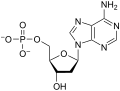
\includegraphics[width=0.9\linewidth]{nucleotide.pdf}
		\caption{Nucleotide formato a sinistra da un gruppo fosfato contenente un atomo di fosforo \ce{P} (che determina il carattere acido degli acidi nucleici), al centro da uno zucchero (desossiribosio) formato da cinque atomi di carbonio e in alto a destra da una base azotata contenente un gruppo \ce{\bond{-}NH} (che conferisce loro un carattere basico) legata con lo zucchero per mezzo di un legame glicosidico.(a sinistra)o zucchero cinque (cita
			%https://en.wikipedia.org/wiki/Nucleotide
			).}
		\label{fig:nucleotide}
	\end{figure}
	
	Oltre al DNA esiste anche l'RNA (acido ribonucleico), un acido nucleico fondamentale per la biosintesi delle proteine. Nonostante DNA e RNA siano entrambi costituiti da una lunga catena nucleotidica, presentano varie differenze strutturali e funzionali:
	\begin{itemize}
		\item il DNA ha una struttura di doppia elica (caratterizzata dal diametro costante di $2\mbox{ nm}$ (cita
		%libro 3 anno CAMPBELL
		)) costituita da due catene nucleotidiche antiparallele (legate tramite legami idrogeno che intercorrono tra A e T oppure tra C e G), mente l'RNA è formato da una singola elica in cui la timina (T) viene sostituita dall'uracile (U) (\hyperref[fig:dna_structure]{Fig. 1.9});
		\item lo zucchero del DNA (desossiribosio) possiede un atomo di ossigeno in meno rispetto al ribosio dell'RNA;
		\item nelle cellule eucariote, il DNA è collocato nel nucleo mentre l'RNA si trova sia nel nucleo che nel citoplasma;
		\item il DNA è depositario dell'informazione genetica mentre l'RNA è l'intermediario tra il DNA e la sintesi di proteine specifiche.
	\end{itemize}
	La scoperta delle strutture degli acidi nucleici DNA e RNA (\hyperref[fig:dna_structure]{Fig. 1.9}) viene attribuita agli scienziati James D. Watson ($1928$--), Francis H. C.Crick ($1916$--$2004$) e Maurice H. F. Wilkins ($1916$--$2004$) che per il loro contributo alla biologia molecolare ricevettero il premio Nobel per la fisiologia o la medicina nel $1958$. In realtà la prima immagine cristallografica del DNA fu quella della chimica Rosalind E. Franklin ($1920$--$1958$), anche se per molto tempo non gli fu riconosciuta la paternità della scoperta. Purtroppo la sua morte precoce non le consentì nemmeno di essere candidata al premio Nobel (cita
	%libro 3 anno CAMPBELL
	).
	
	\begin{figure}[H]
		\centering
		\includegraphics[width=0.9\linewidth]{dna_structure.pdf}
		\caption{Struttura a singola elica dell'RNA e a doppia elica del DNA con relativi accoppiamenti delle basi azotate (cita
		%https://it.wikipedia.org/wiki/Acidi_nucleici
		).}
		\label{fig:dna_structure}
	\end{figure}
	
	Come parzialmente accennato in precedenza, le funzioni del DNA sono quelle di regolare la riproduzione delle cellule (mediante la sua duplicazione che favorisce la trasmissione delle informazioni ereditarie) e di controllare l'espressione genica. In particolare, il dogma centrale della biologia molecolare (proposto nel $1956$ dallo stesso Francis Crick (cita
	%libro campbell3 anno
	)) prevede che le fasi principali della sintesi proteica siano la trascrizione e la traduzione (\hyperref[fig:dna_rna]{Fig. 1.10}). Durante la trascrizione si genera un filamento di mRNA (RNA messaggero) le cui basi azotate sono complementari a quelle della molecola di DNA che è utilizzata come stampo. Durante la traduzione avviene un "cambiamento di linguaggio" in cui l'informazione genica contenuta nel DNA (per mezzo dell'mRNA, dell'tRNA (RNA di trasporto) e dei ribosomi) viene tradotta da una sequenza di nucleotidi in una sequenza di amminoacidi, i "mattoni" che costituiscono le proteine. Nello specifico, ad ogni tripletta di basi azotate (denominata codone) corrisponde un amminoacido (la totalità delle $4^3=64$ combinazioni consente di codificare per tutti i 20 amminoacidi esistenti in natura). Eventuali variazioni della sequenza nucleotidica (come la sostituzione, l'inserzione o la delezione di una base azotata) generano le mutazioni che, in mancanza dei meccanismi di controllo cellulare, sono la causa di molti disturbi e malattie ereditarie (cita
	%libro 3 anno biologia campbell
	).
	
	\begin{figure}[H]
		\centering
		\includegraphics[width=0.9\linewidth]{dna_rna.jpg}
		\caption{Meccanismi di trascrizione e traduzione grazie ai quali il genotipo (l'insieme delle informazioni ereditarie di un organismo) controlla il fenotipo (le caratteristiche fisiche di un organismo) (cita
			%https://ms-mms.hubscuola.it/public/4207663/cdi-4207813/01_infog/index.html
			,
			%libro 3 anno campbell biologia
			).}
		\label{fig:dna_rna}
	\end{figure}
	
	Come già anticipato, il DNA è localizzato nel nucleo della cellula\footnote{In realtà esiste il DNA mitocondriale, un particolare tipo di DNA che contiene informazioni genetiche ereditato solo per linea materna (cita
	%libro 2 anno campbell biologia
	), che è situato all'interno dei mitocondri, organuli cellulari in cui avviene la respirazione cellulare.} ed è legato a particolari proteine che formano una struttura fibrosa chiamata cromatina, che al momento della duplicazione cellulare si addensa formando i cromosomi. Dalle considerazioni precedenti, riassunte nella \hyperref[fig:cell]{Fig. 1.11}, si comprende che il DNA occupa solo una minima parte della cellula: solamente il $2$--$3\%$ del volume cellulare è occupato da DNA. Per questo motivo arrecare danni diretti al DNA da parte di radiazione ionizzante è un evento piuttosto raro, ma non trascurabile.
	\begin{figure}[H]
		\centering
		\includegraphics[width=0.9\linewidth]{cell.jpg}
		\caption{Particolari della struttura della cellula eucariote umana (cita
			%https://mydbook.giuntitvp.it/app/books/GIAC90_G9076812D/html/21
			).}
		\label{fig:cell}
	\end{figure}
	
	Quando la radiazione ionizzante colpisce direttamente il DNA, quest'ultimo può subire danni differenti la cui distribuzione dipende dal tipo di radiazione e dall'energia del fascio incidente. In generale, è possibile suddividere i danni in Single Strand Break (SSB) e Double Strand Breaks (DSB) in quanto nei SSB si genera la rottura di un solo filamento nucleotidico della doppia elica del DNA, mentre nei DSB si ha un danneggiamento in entrambe le catene nucleotidiche, come rappresentato in \hyperref[fig:danni_dna]{Fig. 1.12}. Grazie al meccanismo di correzione di bozze enzimi specifici come DNA polimerasi, DNA ligasi e nucleasi riconoscono i nucleotidi fuori posto e li sostituiscono (mediante un meccanismo chiamato riparazione delle anomalie di appaiamento) prima che possano portare a mutazioni genetiche.\footnote{Ricerche hanno dimostrato che difetti ereditari negli enzimi sopra citati sono associati a una forma di cancro al colon, in quanto gli errori che portano al cancro si accumulano nel DNA più velocemente (cita
	%libro campbell II anno biologia
	).} L'efficacia dei metodi di riparazione dipende dalla complessità del danno iniziale: nei SSB la catena danneggiata viene sostituita dagli enzimi osservando le informazioni della catena integra (sfruttando la complementarietà delle basi azotate), mentre nei DSB si hanno danni che non consentono una ricostruzione della doppia elica; infatti, solo in quest'ultimo caso la cellula potrebbe andare incontro o a morte cellulare (danno deterministico voluto in radio e adroterapia per ottenere l'eliminazione di cellule tumorali) o a carcinogenesi (danno stocastico da limitare in radio e adroterapia, la cui insorgenza è legata alle conseguenze a lungo termine dell'esposizione alla radiazione), perdendo in ambo i casi la sua capacità riproduttiva (cita
	%https://fisica.unipv.it/Eventi/Incontri-fisica-moderna/2017-12-12-Baiocco-Babini-slides.pdf
	).
	
	\begin{figure}[H]
		\centering
		\includegraphics[width=0.9\linewidth]{danni_dna.jpg}
		\caption{Schematizzazione dei SSB (a sinistra), dei DSB (al centro) e di cluster di DSB (a destra) (cita
			%https://fisica.unipv.it/Eventi/Incontri-fisica-moderna/2017-12-12-Baiocco-Babini-slides.pdf
			).}
		\label{fig:danni_dna}
	\end{figure}
	
	\subsubsection{Danno indiretto}\label{par:danno_indiretto}
	Per i motivi esposti nel paragrafo precedente, circa i $2/3$ dei danni cellulari si generano utilizzando radiazione ionizzante che non colpisce direttamente il DNA (cita
	%https://www.dkfz.de/en/medizinische-physik-radioonkologie/Teaching/10_LEM_Models_Carbon_RadiobiologicalModeling.pdf
	). Uno dei danni indiretti più frequenti si ha quando la radiazione colpisce l'acqua contenuta nelle cellule cancerose\footnote{Dato che il corpo umano è costituito per il $75\%$ da acqua, irradiare la cellula equivale, di fatto, a irradiare acqua.} producendo radicali liberi\footnote{I radicali liberi sono atomi neutri o molecole che possiedono un unico elettrone spaiato nel loro orbitale più esterno, caratteristica che è fonte di grande instabilità chimica; ciò rende i radicali liberi particolarmente reattivi e in grado sia di legarsi ad altri radicali sia di sottrarre elettroni a molecole vicine (cita
	%Paolo Silvestroni, Fondamenti di chimica, Bologna, Zanichelli, 1996
	).} tramite processi di radiolisi\footnote{Per radiolisi chimica si intende la scissione di uno o più legami causata da radiazioni ionizzanti (cita
	%https://goldbook.iupac.org/terms/view/R05112
	).} dell'acqua. La radiolisi dell'acqua consiste in una serie di reazioni chimiche (alcune delle quali riportate di seguito) che producono elettroni, atomi, molecole e ioni che, diffondendo, danneggiano indirettamente il DNA portando alla morte cellulare. La ionizzazione di una molecola d'acqua (\ce{H2O}) viene riassunta nella \hyperref[eq:radiolisi1]{Eq. 1.1}:
	\begin{equation}
		\ce{H2O ->[Radiazione ionizzante] H2O^{+} + e^-}
		\label{eq:radiolisi1}
	\end{equation}
	da cui si producono uno ione positivo \ce{H2O^{+}} e un elettrone \ce{e^-}. Trascorso un certo intervallo di tempo, alcuni elettroni perdono una buona parte di energia cinetica che rende possibile la cattura elettronica da parte di un'altra molecola d'acqua con conseguente formazione di uno ione negativo \ce{H2O^{-}}, come descritto nella \hyperref[eq:radiolisi2]{Eq. 1.2}:
	\begin{equation}
		\ce{H2O + e^{-} ->[Cattura elettronica] H2O^{-}}
		\label{eq:radiolisi2}
	\end{equation}
	In seguito i prodotti delle \hyperref[eq:radiolisi1]{Eq. 1.1} e \hyperref[eq:radiolisi2]{Eq. 1.2} si dissociano nei seguenti modi:
	\begin{subequations}
		\begin{align}
			\label{eq:dissociazione1}
			\ce{H2O^{+} ->[Dissociazione] H^{+} + OH^{.}}\\
			\label{eq:dissociazione2}
			\ce{H2O^{-} ->[Dissociazione] OH^{-} + H^{.}}
		\end{align}
	\end{subequations}
	i cui prodotti sono gli ioni idrogeno \ce{H^{+}} e ossidrile \ce{OH^{-}} e i radicali liberi ossidrile \ce{OH^{.}} e idrogeno \ce{H^{.}}. Tra le varie reazioni chimiche che possono avvenire successivamente, i cui reagenti sono i prodotti delle \hyperref[eq:dissociazione1]{Eq. 1.3a} e \hyperref[eq:dissociazione2]{Eq. 1.3b}, si riportano le seguenti:
	\begin{subequations}
		\begin{align}
			\label{eq:prodotto1}
			\ce{H^{.} + OH^{.} &-> H2O}\\
			\label{eq:prodotto2}
			\ce{H^{+} + OH^{-} &-> H2O}\\
			\label{eq:prodotto3}
			\ce{2OH^{.} &-> H2O2}
		\end{align}
	\end{subequations}
	Le \hyperref[eq:prodotto1]{Eq. 1.4a} e \hyperref[eq:prodotto2]{Eq. 1.4b} sono reazioni innocue in quanto generano molecole d'acqua mentre la \hyperref[eq:prodotto3]{Eq. 1.4c} porta alla formazione di perossido di idrogeno (acqua ossigenata, \ce{H2O2}), una sostanza nociva per la cellula in quanto capace di modificare la struttura e le funzioni delle proteine, di mutare le basi nucleotidiche e di generare SSB nel DNA (cita
	%https://www.rndsystems.com/resources/articles/reactive-oxygen-species-ros
	). Ciò spiega il motivo per cui i danni indiretti al DNA, per mezzo della catena di radiolisi dell'acqua, portino la cellula alla morte riproduttiva (cita
	%https://www.mdpi.com/2073-4441/3/1/235
	).
	
	Il corpo umano attua una catena di meccanismi di difesa in presenza di \ce{H2O2} (e altre specie chimiche come i due radicali anione superossido \ce{O2^{-.}} e ossidrile \ce{OH^{.}}, generalmente denominate ROS (Specie Reattive all'Ossigeno)) che si attivano in maniera naturale durante le reazioni di riduzione dell'ossigeno ad acqua, da cui i mitocondri cellulari ricavano energia per il corpo umano. Il primo meccanismo di difesa è quello di disattivare il radicale \ce{O2^{-.}} tramite l'enzima superossido dismutasi (SOD), che catalizza la reazione \hyperref[eq:sod]{Eq. 1.5}:
	\begin{equation}
		\ce{2O2^{-.} + 2H^+ ->[SOD] H2O2 + O2}
		\label{eq:sod}
	\end{equation}
	in cui l'anione superossido viene trasformato in perossido di idrogeno. Successivamente, per disattivare il perossido di idrogeno, intervengono gli enzimi glutatione perossidasi e catalasi che catalizzano rispettivamente le reazioni \hyperref[eq:gsh]{Eq. 1.6a} e \hyperref[eq:catalasi]{Eq. 1.6b}:
	\begin{subequations}
		\begin{align}
			\label{eq:gsh}
			\ce{2GSH + H2O2 &->[Glutatione perossidasi] 2H2O + GSSG}\\
			\label{eq:catalasi}
			\ce{2H2O2 &->[Catalasi] 2H2O + O2}
		\end{align}
	\end{subequations}
	dove \ce{GSH} e \ce{GSSG} sono rispettivamente la forma ridotta e la forma ossidata del glutatione (il substrato\footnote{Il substrato di un enzima è un reagente specifico su cui agisce l'enzima stesso al fine di catalizzare una certa reazione chimica (cita
		%libro campbell 2 anno biologia
		).} della glutatione perossidasi) e \ce{O2} è una molecola di ossigeno.
	
	Anche le sostanze antiossidanti, come la vitamina E, consentono di catturare i radicali liberi diminuendo la loro azione dannosa. In generale, gli enzimi glutatione perossidasi e catalasi e la vitamina E hanno una concentrazione maggiore nei luoghi in cui il danno da ROS tende a essere maggiore, per esempio nei siti più ossigenati. Infatti, osservando l'\hyperref[eq:sod]{Eq. 1.5}, l'eccesso di ossigeno nei tessuti amplifica i danni dovuti all'\ce{H2O2} (si veda \hyperref[par:oer]{OER}) (cita
	%https://www.rndsystems.com/resources/articles/reactive-oxygen-species-ros
	,
	%Ugo Leuzzi, Ersilia Bellocco e Davide Barreca, Biochimica della nutrizione, ISBN 978-88-08-17926-5.
	). In conclusione, meccanismi di difesa come quelli sopra citati riescono a mantenere un equilibrio tra la produzione e la distruzione di radicali liberi dell'organismo umano, ma l'applicazione di una radiazione ionizzante esterna è in grado di generare un disequilibrio che, eventualmente, porta alla morte della cellula.
	
	\subsection{Grandezze dosimetriche}
	In radiobiologia la dosimetria definisce e quantifica le grandezze che descrivono l'interazione delle radiazioni ionizzanti con la materia e gli effetti biologici dell'assorbimento radiativo da parte dei tessuti del corpo umano. Nel TP dei pazienti affetti da neoplasie gli studi dosimetrici sono fondamentali in quanto consentono di misurare la quantità di radiazione necessaria all'eliminazione del tumore e i danni biologici arrecati all'organismo. Nei prossimi paragrafi si espongono le principali grandezze fisico-biologiche utilizzate in dosimetria, molte delle quali sono definite dall'ICRU (International Commission on Radiation Units and Measurements) (cita
	%https://web.archive.org/web/20130929015325/http://icru.org/pdf/icru_poster.pdf
	).
	
	\subsubsection{Dose assorbita, equivalente ed efficace}
	Tra le grandezze dosimetriche caratteristiche della sorgente si trova la fluenza di particelle $\phi$, definita come il numero di particelle $dN$ (ad esempio i protoni all'interno di un fascio) per unità di superficie perpendicolare alla direzione del fascio $dS$. La fluenza è espressa nella sua forma differenziale nella \hyperref[eq:fluence]{Eq. 1.7}:
	\begin{equation}
		\phi=\frac{dN}{dA}
		\label{eq:fluence}
	\end{equation}
	Dalla fluenza di particelle è definibile la dose assorbita $D_{as}$ ossia l'energia assorbita $dE$ assorbita per unità di massa $dm$:
	\begin{equation}
		D_{as}=\frac{dE}{dm}=\frac{\left(\frac{dE}{dx}\right)\Delta x N}{\rho \Delta x A}=\phi\frac{\left(\frac{dE}{dx}\right)}{\rho}
		\label{eq:dose_as}
	\end{equation}
	dove $\left(\frac{dE}{dx}\right)$ è il potere frenante (energia persa dal fascio di particelle per unità di distanza percorsa nel mezzo irradiato, si veda \hyperref[eq:bethe_bloch]{Eq. 1.35}), $N$ è il numero di particelle del fascio e $\rho$ è la densità di massa volumetrica del materiale irradiato. L'unità di misura della dose nel SI (Sistema Internazionale) è il Gray (Gy), tale che $1\mbox{ Gy}=1\frac{J}{kg}$. La dose assorbita è la grandezza dosimetrica per antonomasia in quanto consente di rappresentare la distribuzione della quantità di energia radiativa ricevuta dal paziente durante la terapia per unità di massa del tessuto; nonostante ciò, la $D_{as}$ non tiene conto dei diversi effetti biologici che possono essere indotti da fasci radiativi di tipo differente. Infatti, a parità di dose assorbita, il danno biologico può variare in base all'energia assorbita dal mezzo irradiato per unità di percorso (LET, si veda \hyperref[par:let]{Linear Energy Transfer}), all'Efficacia Biologica Relativa (RBE, si veda \hyperref[??]{??}) che quantifica la variabilità degli effetti biologici dovuta a radiazioni con differente LET e all'abbondanza di ossigeno nei tessuti (si veda \hyperref[par:oer]{OER}) (cita
	%note dal corso di fisica biomedica a.a. 2022-2023
	). Pertanto, per includere i diversi effetti biologici dovuti a tutti i possibili tipi di radiazione $R$, si introduce la dose equivalente $D_{eq}$ definita dalla \hyperref[eq:dose_eq]{Eq. 1.9}:
	\begin{equation}
		D{eq}=\sum_{R}w_RD_{as,R}
		\label{eq:dose_eq}
	\end{equation}
	dove $D_{as,R}$ è la dose assorbita relativa alla radiazione $R$-esima e $w_R$ pondera la pericolosità della radiazione. $w_R$, denominato fattore di qualità, è un numero puro dato dal rapporto tra il danno biologico prodotto dall'assorbimento di $1\mbox{ Gy}$ della radiazione $R$ e il danno biologico prodotto da $1\mbox{ Gy}$ di raggi $\gamma$: $w_R=\frac{Danno(R)}{Danno(\gamma)}$. La prima unità di misura della dose equivalente fu il rem (röntgen equivalent man), oggi sostituito dal Sievert (Sv), tale che $1\mbox{ Sv}=100\mbox{ rem}$. La $D{eq}$ è una grandezza ancora incompleta in quanto non quantifica gli effetti biologici in relazione al tipo di organo o tessuto irradiato. Pertanto si definisce la dose efficace $D_{eff}$ che comprende sia gli effetti biologici dovuti al tipo di radiazione $R$ sia quelli legati a tutti i tessuti e organi irradiati $T$. La dose efficace è definita dalla \hyperref[eq:dose_eff]{Eq. 1.10}:
	\begin{equation}
		D_{eff}=\sum_{T}w_TD_{eq}=\sum_{T}w_T\sum_{R}w_RD
		\label{eq:dose_eff}
	\end{equation}
	dove $w_T$ è un fattore di ponderazione per il tessuto $T$-esimo tale che $\sum_{T}w_T=1$, dove la somma avviene su tutti gli organi e i tessuti del corpo umano considerati sensibili all'induzione di effetti stocastici provocati dalla radiazione. In particolare, $w_T$ è maggiore per i tessuti più sensibili alla radiazione\footnote{I tessuti più sensibili alla radiazione sono quelli in cui è più facile rimuovere le cellule neoplastiche, ma sono anche i tessuti più soggetti all'insorgenza di effetti collaterali dovuti all'applicazione di radiazione ionizzante.} come quelli caratterizzati da un'elevata riproduzione cellulare, in cui l'eliminazione del cancro ha una maggiore riuscita. Anche la $D_{eff}$ si misura in Sievert, in modo che gli effetti biologici di $1\mbox{ Sv}$ di una data radiazione siano uguali a quelli di $1\mbox{ Gy}$ dei raggi $\gamma$, presi come riferimento. Si riportano alcuni valori di $w_R$ e $w_T$ in \hyperref[tab:w_factor]{Tab. 1.1}.
	
	\begin{table}[H]
		\begin{minipage}{\textwidth}
			\centering
			\begin{tabular}{ |m{10.5cm}||M{3.5cm}| }
				\hline
				Tipo di radiazione & $w_R$ \\
				\hline\hline
				Fotoni & 1\\
				\hline
				Elettroni e muoni & 1\\
				\hline
				Protoni e pioni carichi & 2\\
				\hline
				Particelle alfa, frammenti di fissione, nuclei pesanti & 20\\
				\hline\hline
				Organi o tessuti & $w_T$\\
				\hline\hline
				Gonadi & 0.08 \\
				\hline
				Midollo osseo (rosso) & 0.12\\
				\hline
				Colon & 0.12\\
				\hline
				Polmone (vie respiratorie toraciche) & 0.12\\
				\hline
				Stomaco & 0.12\\
				\hline
				Mammelle & 0.12\\
				\hline
				Vescica & 0.04\\
				\hline
				Fegato & 0.04\\
				\hline
				Esofago & 0.04\\
				\hline
				Tiroide & 0.04\\
				\hline
				Pelle & 0.01\\
				\hline
				Superficie ossea & 0.01\\
				\hline
				Cervello & 0.01\\
				\hline
				Ghiandole salivari & 0.01\\
				\hline
				Rimanenti organi o tessuti\footnote{Ghiandole surrenali, regione extratoracica, vescichetta biliare, cuore, reni, linfonodi, muscolo, mucosa orale, pancreas, prostata (uomini), intestino tenue, milza, timo, utero/collo dell'utero (donne).} & 0.12\\
				\hline
			\end{tabular}
		\end{minipage}
		\caption{Tabella riassuntiva dei valori di alcuni fattori di ponderazione per la radiazione $w_R$ e per organi e tessuti $w_T$ (cita
				%pdf D.Lgs. 101-2020 in \Tesi\FOOT\Materiale
				).}
		\label{tab:w_factor}
	\end{table}
	
	\subsubsection{Linear Energy Transfer}\label{par:let}
	Il Linear Energy Transfer (LET) di una radiazione ionizzante è la quantità di energia $dE$ trasferita al materiale a causa delle collisioni per unità di distanza $dx$:
	\begin{equation}
		LET=\frac{dE_\Delta}{dx}
		\label{eq:let}
	\end{equation}
	Già nella \hyperref[eq:dose_as]{Eq. 1.8} viene utilizzato il potere frenante $\left(\frac{dE}{dx}\right)$, simile alla definizione di LET. Il motivo per cui tali termini si trattano separatamente risiede in una loro differenza: mentre il potere frenante è legato all'energia persa dal fascio di particelle nel mezzo che attraversa (per unità di distanza), il LET si riferisce all'energia assorbita dal mezzo (per unità di distanza). Nella \hyperref[eq:let]{Eq. 1.11} compare il pedice $\Delta$ in quanto nella definizione di LET si tengono conto dei trasferimenti di energia localizzati vicino alla traiettoria della particella, escludendo le ionizzazioni degli elettroni a lungo raggio più energetici la cui energia è maggiore di una soglia $\Delta$ come illustrato in \hyperref[fig:let]{Fig. 1.13}. Nel limite $\Delta\rightarrow+\infty$\footnote{Tale condizione limite non si raggiunge fisicamente, ma corrisponde al caso in cui vengono inclusi tutti i trasferimenti di energia della \hyperref[eq:let]{Eq. 1.11}, per quanto grandi possano essere.} non esisterebbero più elettroni con $E>\Delta$ in quanto l'energia persa dalla particella del fascio corrisponderebbe eguaglierebbe l'energia assorbita dal materiale (il che renderebbe equivalenti il potere frenante e il LET). Tali considerazioni consentono di ricavare la relazione che lega il potere frenante e il LET:
	\begin{equation}
		LET=\frac{dE_\Delta}{dx}-K_{E>\Delta}
		\label{eq:let&stoppingpower}
	\end{equation}
	dove $K_{E>\Delta}$ è l'energia cinetica degli elettroni che possiedono un'energia $E>\Delta$.
	
	\begin{figure}[H]
		\centering
		\includegraphics[width=0.9\linewidth]{let.jpg}
		\caption{Il cilindro schematizza la traiettoria di una particella del fascio. Gli elettroni $e_1$ ed $e_2$ possiedono energie rispettivamente $E_1>\Delta$ ed $E_2<\Delta$. Nella definizione di LET si considerano solo gli elettroni a corto raggio come $e_2$.}
		\label{fig:let}
	\end{figure}
	
	In base al LET è possibile distinguere due tipi di radiazione, quelle ad alto e basso LET. Le radiazioni a basso LET, disperdendo poca energia nei tessuti per unità di percorso, penetrano più in profondità rispetto alle radiazioni ad alto LET in quanto impiegano più tempo a esaurire l'energia che possiedono. Inoltre le radiazioni ad alto LET arrecano danni biologici maggiori ai tessuti in quanto generano eventi di ionizzazione più frequenti e ravvicinati. La \hyperref[fig:damage_let]{Fig. 1.14} mostra che le radiazioni a basso LET, per esempio raggi X o $\gamma$, inducono prevalentemente danni isolati al DNA come le SSB mentre radiazioni ad alto LET, tra cui si trovano le particelle $\alpha$ o gli ioni pesanti, generano danni più distruttivi al DNA come le DSB (cita
	%https://www.ncbi.nlm.nih.gov/pmc/articles/PMC7555951/	
	).
	
	\begin{figure}[H]
		\centering
		\includegraphics[width=0.9\linewidth]{damage_let.png}
		\caption{Danni tipici del DNA da parte di radiazioni a basso LET (in alto) e ad alto LET (in basso) (cita
			%https://www.cambridge.org/core/journals/expert-reviews-in-molecular-medicine/article/cell-death-mechanisms-in-head-and-neck-cancer-cells-in-response-to-low-and-highlet-radiation/5D81C15D79DA4C3B485D4367D5C7CBD3
			).}
		\label{fig:damage_let}
	\end{figure}
	
	Dalla \hyperref[fig:proton_carbon_let]{Fig. 1.15} si osserva che i fasci adroterapici di protoni e ioni carbonio rilasciano una dose di energia sempre maggiore nel materiale in cui penetrano, fin quando non si verifica un picco di perdita di energia in corrispondenza del picco di Bragg, dopo il quale le particelle si fermano. Tale decelerazione, che avviene in maniera approssimativamente continua fino al BP, causa una variazione nella sezione d'urto delle particelle \hyperref[sez]{sez d'urto ref} che incrementa gli eventi di ionizzazione all'interno del materiale: per tale motivo si osserva un aumento di LET durante il percorso delle particelle, che raggiunge un massimo in corrispondenza del BP. Inoltre, considerando livelli energetici terapeutici, si nota che gli ioni carbonio possiedono valori di LET più alti rispetto a quelli dei protoni (si veda la \hyperref[tab:let_rbe]{Tab. 1.2}) poiché i primi possiedono una carica maggiore dei secondi che gli consente di effettuare molte più interazioni a parità di distanza percorsa in grado di generare ingenti danni come le DSB, specialmente nella regione del BP (\hyperref[tab:let_rbe]{Tab. 1.2}).
	
	\begin{figure}[H]
		\centering
		\includegraphics[width=0.9\linewidth]{proton_carbon_let.jpg}
		\caption{Distribuzione microscopica delle ionizzazioni adroniche in scala nanometrica con relativo LET, profondità raggiunta, energia cinetica e distanza media della creazione del danno (cita
			%Slide Spighi L01
			).}
		\label{fig:proton_carbon_let}
	\end{figure}
	
	In \hyperref[fig:proton_carbon_let]{Fig. 1.15} si nota che nel canale di ingresso, che corrisponde alla prima parte della penetrazione dove il rilascio di dose è minore, i protoni e gli ioni carbonio effettuano un danno rispettivamente ogni $90 \mbox{ nm}$ (insufficiente a colpire la doppia catena del DNA, il cui diametro è di $2 \mbox{ nm}$) e ogni $4 \mbox{ nm}$ (sufficiente a generare SSB), mentre in corrispondenza del BP i protoni e gli ioni carbonio effettuano un danno rispettivamente ogni $4 \mbox{ nm}$ e ogni $0.3 \mbox{ nm}$ (sufficienti a generare rispettivamente SSB e DSB). Pertanto gli ioni carbonio sono più dannosi dei protoni in prossimità del BP, ma nel canale di ingresso causano molti più danni dei protoni; tale discordanza va tenuta conto in fase di TP affinché si selezioni il fascio adroterapico più adeguato alle specificità tessutali del paziente.
	
	\subsubsection{Relative Biological Effectiveness}\label{par:rbe}
	La Relative Biological Effectiveness (RBE) di una radiazione ionizzante $R$ è un numero puro dato dal rapporto tra la dose $D_\gamma$ rilasciata dai raggi $\gamma$ e la dose $D_R$ rilasciata da $R$ al fine di ottenere lo stesso effetto biologico, fissato il tasso di sopravvivenza delle cellule $S$:
	\begin{equation}
		RBE=\frac{D^S_\gamma}{D^S_R}
		\label{eq:rbe}
	\end{equation}
	Ad esempio, se una radiazione $R$ ha $RBE>1$ significa che è necessaria una dose minore di $R$ per ottenere gli stessi danni biologici dei raggi $\gamma$ (in altre parole la radiazione $R$ è più efficace dei raggi $\gamma$). La valutazione dell'RBE è piuttosto complessa in quanto dipende dal tipo di radiazione, dall'energia della radiazione, dall'LET (\hyperref[fig:let_rbe]{Fig. 1.16a}), dal tipo di cellula e dal rateo di sopravvivenza della cellula (\hyperref[fig:survival_dose]{Fig. 1.16b}); in \hyperref[tab:let_rbe]{Tab. 1.2} vengono riportati valori di RBE per alcuni tipi di radiazione.
	
	\begin{figure}[H]
		\centering
		\begin{subfigure}[t]{0.49\textwidth}
			\centering
 			\includegraphics[width=\textwidth, scale=0.5]{let_rbe1.png}
			\caption{RBE in funzione dell'LET per cellule T1 renali umane irradiate con particelle pesanti cariche mono-energetiche. Le curve $1$, $2$ e $3$ corrispondono all'RBE misurato con frazioni di sopravvivenza cellulare di $0.8$, $0.1$, $0.01$ (cita
				%https://www.mdpi.com/2073-4468/1/2/124
				).}
			\label{fig:let_rbe}
		\end{subfigure}
		\hfill
		\begin{subfigure}[t]{0.49\textwidth}
			\centering
			\includegraphics[width=\textwidth, scale=0.5]{survival_dose.jpg}
			\caption{Curve di sopravvivenza cellulare per fotoni e ioni in funzione della dose rilasciata e determinazione dell'RBE fissati i livelli di sopravvivenza del $10\%$ e dell'$1\%$ (cita
				%https://radiologykey.com/radiation-therapy-with-protons-and-heavy-ions/
				).}
			\label{fig:survival_dose}
		\end{subfigure}
		\caption{Andamento dell'RBE in funzione dell'LET e del tasso di sopravvivenza della cellula.}
	\end{figure}
		
	\begin{table}[H]
		\centering
		\begin{tabular}{ |m{10cm}||M{3cm}|M{1cm}| }
			\hline
			Tipo di radiazione & LET $\left[\mbox{keV/}\mu\mbox{m}\right]$ & RBE\\
			\hline\hline
			Raggi X ($6$--$15 \mbox{ MeV}$) & $0.3$ &	$\approx 0.8$\\
			\hline
			Particella $\beta$ ($1 \mbox{ MeV}$) & $0.3$ & $0.9$\\
			\hline
			Raggi $\gamma$ ($1 \mbox{ MeV}$) & $0.5$ & $1$\\
			\hline
			Protoni a energie terapiche ($150 \mbox{ MeV}$) & $0.5$ & $\approx1.1$\\
			\hline
			Neutroni & $0.5$--$100$ & $1$--$2$\\
			\hline
			Particella $\alpha$ & $50$--$200$ & $5$--$10$\\
			\hline
			Ioni carbonio nella regione vicina al picco di Bragg & $40$--$90$ & $2$--$5$\\
			\hline
		\end{tabular}
		\caption{Valori approssimati di LET e RBE di alcuni tipi di radiazione (cita
			%Hasan Murshed M.D., M.S, in Fundamentals of Radiation Oncology (Third Edition), 2019
			,
			%P. Dendy & B. Heaton, Physics for Diagnostic Radiology, 2nd Edition
			).}
		\label{tab:let_rbe}
	\end{table}
	
	Dalla \hyperref[tab:let_rbe]{Tab. 1.2} si nota che i fasci adroterapici di ioni carbonio sono molto più efficienti dei fasci radioterapici fotonici (raggi $\gamma$). I protoni, invece, possiedono un RBE solo del $10\%$ più grande rispetto ai fotoni; tale somiglianza non sembrerebbe coadiuvare le riflessioni esposte nella \hyperref[sec:1.2]{Sez. 1.2}, in cui si sono evidenziati i grandi vantaggi della protonterapia sulla radioterapia in relazione alla cure dei tumori più profondi. In realtà l'efficienza protonterapica vince su quella radioterapica se si tengono conto degli effetti globali di entrambe le radiazioni: mentre i protoni (così come gli ioni carbonio) rilasciano la maggior parte della dose in una zona ristretta situata in prossimità del picco di Bragg, i fotoni rilasciano la dose in una regione molto più ampia, come evidenziato nella \hyperref[fig:photon]{Fig. 1.17}.
	
	\begin{figure}[H]
		\centering
		\includegraphics[width=0.9\linewidth]{photon.jpg}
		\caption{Rilascio di dose relativa in funzione della profondità del tessuto per fotoni, elettroni, ioni carbonio e protoni. Si notino i picchi di Bragg sia per gli ioni carbonio che per i protoni (particelle usate in adroterapia), assenti per elettroni e fotoni (particelle usate in radioterapia) (cita
			%https://www.mdpi.com/2227-9059/9/1/31
			).}
		\label{fig:photon}
	\end{figure}
	
	Negli ultimi anni la variabilità dell'RBE protonico è stata ampiamente dibattuta in quanto vi sono misure radiobiologiche che attestano valori superiori rispetto all'$1.1$ riportato in \hyperref[tab:let_rbe]{Tab. 1.2} (cita
	%J. Tang et al., “Comparison of radiobiological effective depths in 65-MeV modulated proton beams.,” 1992 Brit. J. Cancer, vol. 76, no. 2, p. 220, 1997.
	). Nella ref. (cita
	%F. Tommasino and M. Durante, “Proton radiobiology,” Cancers, vol. 7, no. 1, pp. 353–381, 2015.
	) si propone che l'aumento dell' RBE protonico sia causato dalle particelle prodotte nella frammentazione del target\footnote{In fisica nucleare e subnucleare il target (o targhetta) è una porzione di materia che funge da bersaglio di un fascio di particelle inviato per studiare la materia, il fascio e le loro interazioni (cita
		%https://www.treccani.it/enciclopedia/target/
		).}: nell'attraversare il paziente, le interazioni nucleari che intercorrono tra il fascio protonico e i tessuti del paziente stesso generano dei frammenti, particelle secondarie caratterizzate da un corto raggio ($10$--$100\mu\mbox{ m}$), alto LET e conseguentemente alto RBE. Uno degli obiettivi primari dell'esperimento FOOT (si veda \hyperref[ref a capitolo 2]{?ref a capitolo 2?}) è proprio quello di migliorare l'accuratezza dell'RBE protonico (in funzione di profondità e tipo di tessuto) a partire da misure di sezioni d'urto differenziali, energie e direzioni dei frammenti; conoscere minuziosamente tali grandezze porterebbe a valutazioni più precise degli effetti biologici protonterapici che ridurrebbero i margini di errore in fase di TP.
		
	Nel corso del tempo molti studi si sono incentrati sul legame tra RBE e LET, fortemente dipendente dalla natura del materiale biologico e dalla scelta dell'endpoint utilizzato per definire l'efficacia radioterapica. Pur fissando tali parametri, alcuni risultati mostrano che radiazioni differenti aventi stessi LET possiedono diversi RBE (cita
	%International Commission on Radiation Units and Measurements (1970). Linear Energy Transfer. Washington D.C. doi:10.1093/jicru/os9.1.Report16. ISBN 978-0913394090. ICRU report 16.
	). Nonostante ciò, la \hyperref[fig:let_rbe]{Fig. 1.16a} riporta un tipico andamento di RBE e LET in cui si osserva che l'RBE aumenta al crescere dell'LET fino a raggiungere un massimo intorno ai $100\mbox{keV}/\mu\mbox{m}$, dopo il quale si verifica una forte diminuzione. La spiegazione del primo tratto è ovvia, in quanto più energia assorbe il materiale attraversato da radiazione più danni biologici saranno arrecati allo stesso, mentre nel secondo tratto si verifica un fenomeno di saturazione denominato overkill cellulare in cui la quantità di energia che viene depositata è così elevata che si produce una quantità di danni al DNA maggiore di quella richiesta per la morte cellulare, da cui consegue la riduzione dell'efficacia biologica del trattamento (
	%Linz U, editor. Ion beam therapy: fundamentals, technology. In: Clinical applications. Berlin: Springer; 2012.
	).
	
	Comprendere quale sia il range di dose più efficace nei trattamenti radio e adroterapici è molto complesso in quanto gli effetti radiobiologici dipendono da molti parametri, alcuni dei quali vengono analizzati nei paragrafi successivi. In generale, durante il TP dei pazienti affetti da tumore, sono due i fattori che influenzano la scelta della dose: il TCP (Tumor Control Probability) e l'NTCP (Normal Tissue Complication Probability). Lo scopo di radio e adroterapia è quello di raggiungere un'elevata probabilità di controllare localmente un tumore (che corrisponde a un alto valore di TCP) mantenendo bassa la probabilità di sviluppare complicazioni nei tessuti sani (che corrisponde all'NTCP) (cita
	%Baumann M, Petersen C. TCP and NTCP: a basic introduction. Rays. 2005 Apr-Jun;30(2):99-104. PMID: 16294901.
	). Teoricamente, il range di dose più efficiente è quello che massimizza il TCP e minimizza l'NTPC (in altre parole il range di dose ottimale è quello che massimizza la differenza tra TCP e NTCP). Dato che le cellule sane sono in grado di riparare i danni radiativi meglio delle cellule cancerose, tale range esiste (pur essendo fortemente dipendente dal tipo di tumore e dal suo stadio) e si attesta intorno a $20$--$80\mbox{ Gy}$, valori letali se rilasciati in un'unica seduta (questo è uno dei motivi per cui si effettua il frazionamento, si veda \hyperref[sec:sopravvivenza_cellulare]{Sez. 1.4.3}). Chiaramente, si fornisce un intervallo di valori in quanto la dose dipende dal tipo di tumore e dal suo stadio. Tali considerazioni sono riassunte in \hyperref[fig:tcp]{Fig. 1.18} .
	
	\begin{figure}[H]
		\centering
		\includegraphics[width=0.9\linewidth]{tcp.jpg}
		\caption{Andamenti del TCP (in verde), dell'NTCP (in rosso), della loro differenza (in blu) e dell'assenza di complicazioni nei tessuti sani (in nero) in funzione della dose rilasciata nei tessuti. Il range di dose ottimale nei trattamenti si trova in corrispondenza della curva blu (cita
			%https://link.springer.com/chapter/10.1007/978-3-030-02958-6_12
			).}
		\label{fig:tcp}
	\end{figure}

	\subsubsection{Oxygen Enhancement Ratio}\label{par:oer}
	L'Oxygen Enhancement Ratio (OER) è un numero puro che misura l'efficacia biologica della radiazione in relazione alla concentrazione di ossigeno presente nei tessuti. Infatti, come già riportato nell'analisi del \hyperref[par:danno_indiretto]{Danno indiretto} della radiolisi dell'acqua, se il tessuto colpito con radiazione ionizzante presenta un'abbondanza di ossigeno (iperossia) si genera un numero maggiore di radicali liberi e aumentano le possibilità di danno al DNA del tessuto irradiato, come mostrato in \hyperref[fig:oer_survival]{Fig. 1.19}. L'OER è definito come il rapporto tra la dose di una certa radiazione in condizioni di mancanza di ossigeno (anossia) e la dose della stessa radiazione in normali concentrazioni di ossigeno:
	\begin{equation}
		OER=\frac{D_{anossia}}{D_{normale}}
		\label{eq:oer}
	\end{equation}
	
	\begin{figure}[H]
		\centering
		\includegraphics[width=0.9\linewidth]{oer_survival.png}
		\caption{A parità di percentuale di cellule sopravvissute, per arrecare danni biologici in condizioni aerobiche (presenza di ossigeno) è necessaria una dose inferiore rispetto alle condizioni di anossia; maggiore è la concentrazione di ossigeno, maggiore è la probabilità di effettuare dei danni (cita
			%https://en.wikipedia.org/wiki/Oxygen_effect
			).}
		\label{fig:oer_survival}
	\end{figure}
	
	L'OER decresce all'aumentare dell'LET della radiazione ionizzante, come evidenziato in \hyperref[fig:let_oer]{Fig. 1.20a}. Nelle radiazioni a basso LET si verificano eventi di ionizzazione isolati che favoriscono la \hyperref[eq:prodotto1]{Eq. 1.4a}, da cui si ottiene un'innocua molecola d'acqua (\ce{H2O}); per questo motivo l'aggiunta di atomi di ossigeno aumenta notevolmente i danni biologici arrecati ai tessuti e il valore dell'OER si attesta attorno a $2$--$4$. Al contrario, nelle radiazioni ad alto LET si verificano eventi di ionizzazione frequenti che favoriscono la \hyperref[eq:prodotto2]{Eq. 1.4b}, da cui si ottiene una dannosa molecola di perossido di idrogeno (\ce{H2O2}); per questo motivo l'aggiunta di atomi di ossigeno risulta superflua per l'amplificazione dei danni biologici, dato che l'ambiente è già ricco di \ce{H2O2}, e il valore dell'OER si attesta attorno all'unità (cita
	%Elaine M. Zeman, in Clinical Radiation Oncology (Fourth Edition), 2016
	,
	%Barendsen GW. The relationships between RBE and LET for different types of lethal damage in mammalian cells: biophysical and molecular mechanisms. Radiation Res. 1994; 139:257-270.
	). In \hyperref[fig:reaction_let]{Fig. 1.20b} si riassumono le reazioni chimiche favorite in regime di alto e basso LET.
	
	\begin{figure}[H]
		\centering
		\begin{subfigure}[t]{0.49\textwidth}
			\centering
			\includegraphics[width=\textwidth, scale=0.50]{let_rbe2.png}
			\caption{Andamento dell'OER in funzione dell'LET per particelle $\alpha$ mono-energetiche (cita
				%https://www.mdpi.com/2073-4468/1/2/124
				,
				%https://www.uio.no/studier/emner/matnat/fys/FYS4730/v12/undervisningsmateriale/Syllabus.pdf
				).}
			\label{fig:let_oer}
		\end{subfigure}
		\hfill
		\begin{subfigure}[t]{0.49\textwidth}
			\centering
			\includegraphics[width=\textwidth, scale=0.50]{reaction_let.jpg}
			\caption{Schematizzazione delle reazioni più comuni per radiazioni ad alto LET (in alto) e a basso LET (in basso) (cita
				%https://www.mun.ca/biology/scarr/Specific_Ionization_&_LET.html
				).}
			\label{fig:reaction_let}
		\end{subfigure}
		\caption{Rapporto tra l'OER e le radiazioni ad alto e basso LET.}
	\end{figure}
		
	 Spesso accade che la proliferazione di un tumore diventa talmente rapida che il suo apporto di sangue non è sufficiente a ossigenare alcune sue parti, generando microambienti ipossici che rendono il tumore stesso più radioresistente (cita
	 %https://www.ncbi.nlm.nih.gov/pmc/articles/PMC4283800/
	 ) e più incline alla formazione di metastasi (cita
	 %https://pubmed.ncbi.nlm.nih.gov/21593862/
	 ). Per risolvere tale problematica si sono effettuati numerosi approcci sistemici, dal posizionare i pazienti in camere iperbariche prima di procedere con le sedute radioterapiche all'uso di farmaci in grado di incrementare il flusso sanguigno o l'emoglobina\footnote{L'emoglobina è una proteina deputata per il trasporto di ossigeno nel sangue.}, che sono risultati insoddisfacenti in quanto l'omeostasi del corpo umano riesce a mantenere i livelli di ossigeno stabili. Recentemente si sono sviluppati nuovi metodi più efficaci in grado di aumentare localmente la concentrazione di ossigeno, come l'iniezione di "microbolle" nel flusso sanguigno umano (cita
	 %https://www.cancer.gov/news-events/cancer-currents-blog/2018/microbubbles-radiation-breast-cancer
	 ). In generale, tutte le metodiche sopra citate risulterebbero sicuramente utili ad amplificare i danni indiretti al DNA, dall'altra renderebbero più ossigenate anche aree popolate da organi sani, che verrebbero resi più sensibili alla radiazione (cita
	 %https://www.kva.se/en/event/workshop-the-role-of-oxygen-in-radiation-therapy-2/#:~:text=Oxygen%2C%20thus%2C%20is%20one%20of,oxygen%20enhancement%20ratio%20(OER).
	 ).
	
	\subsection{Sopravvivenza cellulare}\label{sec:sopravvivenza_cellulare}
	Dopo aver discusso delle principali grandezze fisico-mediche con cui si valutano gli effetti biologici della radiazione ionizzante è necessario analizzare i modelli che descrivono la sopravvivenza cellulare. Innanzitutto, gli eventi di ionizzazione prodotti dalla radiazione sono processi stocastici. Pertanto la morte cellulare segue leggi probabilistiche dettate dalla statistica di Poisson. Per esempio, consideriamo una dose che, rilasciata una prima volta, riduce la sopravvivenza cellulare del $50\%$; un secondo rilascio ridurrebbe la sopravvivenza al $25\%$, un terzo al $12.5\%$ e così via. Seguendo tale ragionamento, in prima approssimazione è possibile considerare la seguente legge che descrive la frazione di cellule sopravvissute $S$ in funzione della dose rilasciata $D$, mostrata in \hyperref[eq:survival1]{Eq. 1.15}:
	\begin{equation}
		S=e^{-0.69D}
		\label{eq:survival1}
	\end{equation}
	In realtà l'\hyperref[eq:survival1]{Eq. 1.15}, il cui andamento è rappresentato in \hyperref[fig:survival1]{Fig. 1.21a}, descrive il tasso di sopravvivenza per cellule procarioti (come quelle dei batteri), le quali non sono sostanzialmente in grado di riparare i danni radiativi attivando sistemi di riparazione. Al contrario, le cellule degli esseri umani (in generale le cellule eucarioti dei mammiferi) possiedono complessi meccanismi di riparazione del DNA (accennati in \hyperref[par:danno_diretto]{Danno diretto}) che consentono di recuperare i danni dovuti a radiazioni ionizzanti. Suddetti meccanismi, però, sono efficaci solo in presenza di un basso rilascio di dose (basso LET), mentre per alte energie (alto LET) non sono sufficienti a riparare i danni radiativi che risultano addirittura maggiori rispetto a quelli arrecati a cellule batteriche. Pertanto gli effetti dei meccanismi di riparazione incidono nell'andamento della sopravvivenza cellulare solo in un regime di basso LET, come illustrato in \hyperref[fig:survival2]{Fig. 1.21b}.
	
	\begin{figure}[H]
		\centering
		\begin{subfigure}[t]{0.49\textwidth}
			\centering
			\includegraphics[width=\textwidth, scale=0.50]{survival1.jpg}
			\caption{Sopravvivenza cellulare di un batterio Escherichia coli. $D_0$ è la dose che riduce la sopravvivenza di un fattore $1/e$ (cita
				%https://radiologykey.com/5-cell-survival-curves/
				).}
			\label{fig:survival1}
		\end{subfigure}
		\hfill
		\begin{subfigure}[t]{0.49\textwidth}
			\centering
			\includegraphics[width=\textwidth, scale=0.50]{survival2.png}
			\caption{Sopravvivenza cellulare di una cellula di mammifero dopo un irraggiamento ad alto e basso LET. Un rilascio a basso LET arrecano un numero minore di danni che consegue in un appiattimento della pendenza della curva di sopravvivenza indotto dai meccanismi di riparazione del DNA (cita
				%https://www.researchgate.net/publication/23133166_Therapeutic_Radionuclides_Biophysical_and_Radiobiologic_Principles
				).}
			\label{fig:survival2}
		\end{subfigure}
		\caption{Decadimenti esponenziali della sopravvivenza cellulare in funzione della dose in scala semilogaritmica.}
	\end{figure}
	
	In considerazione dell'analisi di cui sopra, l'ICRP (International Commission on Radiological Protection) approvò nel $1991$ un accurato modello radiobiologico in grado di descrivere accuratamente la sopravvivenza cellulare in seguito al rilascio di radiazione ionizzante (cita
	%https://www.icrp.org/publication.asp?id=ICRP%20Publication%2060
	). Tale modello, chiamato LQ (Lineare Quadratico), prevede che la frazione di cellule sopravvissute $S$ in funzione della dose rilasciata $D$ sia descritta dalla \hyperref[eq:survival2]{Eq. 1.16}:
	\begin{equation}
		S=e^{-\alpha D-\beta D^2}
		\label{eq:survival2}
	\end{equation}
	dove $\alpha$ e $\beta$ sono due parametri dipendenti dal tessuto, dalla radiazione e dallo stato di salute cellulare tali che $\left[\alpha\right]\mbox{Gy}^-1$ e $\left[\beta\right]\mbox{Gy}^-2$. In particolare, il fattore lineare $\alpha D$ rappresenta gli eventi di "single hit" in cui il danno cellulare viene provocato da una singola particella incidente, mentre il fattore quadratico $\beta D^2$ rappresenta gli eventi di "multiple hit" in cui il danno cellulare deriva dall'azione di una doppia traccia di particelle (si veda \hyperref[fig:survival_cell]{Fig. 1.22}). In sostanza, $\alpha$ misura la parte dei danni letali non riparabili e rappresenta principalmente gli eventi di DSB, mentre $\beta$ misura la parte dei danni sub-letali\footnote{Un danno sub-letale è un tipo di danno non letali di per sé, ma che combinandosi con ulteriori danni indotti dalle radiazioni può uccidere la cellula (cita
		%https://iopscience.iop.org/article/10.1088/1361-6560/aaf26a/pdf
		).} riparabili e rappresenta maggiormente gli eventi di SSB.
	
	\begin{figure}[H]
		\centering
		\includegraphics[width=0.9\linewidth]{survival_cell.jpg}
		\caption{Andamento della sopravvivenza cellulare in funzione della dose rilasciata. Sinistra: risposte cellulari differenti corrispondenti a diversi valori di $\alpha/\beta$. Le curve con alto $\alpha/\beta=10\mbox{ Gy}$ possiedono tassi quasi costanti di morte cellulare mentre le curve con basso $\alpha/\beta=3\mbox{ Gy}$ mostrano una curvatura pronunciata, con una morte cellulare che aumenta al crescere della dose rilasciata. Destra: separazione della curva di sopravvivenza cellulare in cinetica a singola e a doppia hit. Per basse dosi la cinetica prevalente è quella a singola hit ($S\approx e^{-\alpha}$), mentre a dosi più alte domina la cinetica a hit multipla. Gli effetti di cinetica a singola e a doppia hit sono equivalenti quando $D=\alpha/\beta=5\mbox{ Gy}$ (cita
			%https://iopscience.iop.org/article/10.1088/1361-6560/aaf26a/pdf
			).}
		\label{fig:survival_cell}
	\end{figure}
		
	I modelli di sopravvivenza cellulare per le cellule mammifere e il fatto che le cellule sane recuperano danni più facilmente di quelle cancerose suggeriscono che per eliminare una neoplasia è opportuno effettuare più dosi a bassa energia piuttosto che un'unica dose ad alte energie, in un processo chiamato frazionamento. Tale meccanismo avviene per sfruttare al massimo la capacità riparatrice delle cellule sane, al fine di risparmiare tessuti e organi non malati che, inevitabilmente, vengono colpiti in minima parte nei trattamenti radio e adroterapici (in radioterapia ciò è più frequente che in adroterapia, come mostrano i profili di dose in \hyperref[fig:photon]{Fig. 1.17}). L'intervallo temporale che intercorre tra un rilascio di dose e l'altro non deve essere né troppo breve (si deve evitare che le cellule danneggiate dei tessuti sani vengano uccise dando i giusti tempi di recupero\footnote{Solitamente le cellule sane riparano i danni biologici dopo almeno sei ore (cita
		%https://link.springer.com/chapter/10.1007/978-3-030-61899-5_23
		).}), né troppo lungo (altrimenti l'effetto combinato delle sedute radioterapiche risulterebbe vano rispetto a un unico rilascio di dose). Tipicamente il trattamento radioterapico viene frazionato in $30$--$35$ sedute effettuate giornalmente, in modo che le $24$ ore di attesa tra una seduta e l'altra consentano alle cellule sane di riparare molti più danni rispetto a quelle tumorali, portando lentamente a una riduzione della regione tumorale. Considerando che dosi radiative superiori a $100 \mbox{ Gy}$ potrebbero portare il paziente alla morte e che una dose letale media per una cellula si attesta attorno ai $2 \mbox{ Gy}$, vengono rilasciati circa $1$--$2\mbox{ Gy}$ di dose al volume tumorale per ogni frazione. Per comprendere l'ingenza degli effetti radiativi si pensi che se $1$--$2\mbox{ Gy}$ venissero irradiati sull'intero corpo umano, il paziente impiegherebbe qualche settimana per recuperare appieno le sue condizioni fisiche, mentre un'applicazione di $2$--$6\mbox{ Gy}$ sull'intero corpo umano si rivelerebbe fatale entro due mesi e i pochi sopravvissuti necessiterebbero di circa un anno di recupero.
		
	\subsubsection{Il frazionamento nel modello LQ}
	Il modello LQ risulta particolarmente efficace nell'analizzare il frazionamento. Come analizzato in \hyperref[fig:survival_cell]{Fig. 1.22}, il grado di curvatura della \hyperref[eq:survival2]{Eq. 1.16} è definito in termini del rapporto $\frac{\alpha}{\beta}$. Tipicamente gli organi che contengono cellule che proliferano velocemente (come quelle di pelle, mucosa orale e midollo osseo), denominati early responding, mostrano risposte immediate al trattamento radioterapico e possiedono alti valori di $\frac{\alpha}{\beta}$ (pari a $7$--$10\mbox{ Gy}$) mentre tessuti contenenti cellule che si riproducono più lentamente (come quelle di cuore, polmoni e reni), chiamati late responding, risentono del trattamento radioterapico dopo scale temporali più lunghe (mesi o anni) e possiedono bassi valori di $\frac{\alpha}{\beta}$ (pari a $3$--$5\mbox{ Gy}$). Visto che le neoplasie sono proliferazioni incontrollate di cellule, i tumori appartengono alla classe degli early responding e gli si attribuisce un $\frac{\alpha}{\beta}=10\mbox{ Gy}$. Al contrario, le cellule dei tessuti sani tendono a dividersi più lentamente e, in confronto alle cellule cancerose, possiedono un valore di $\frac{\alpha}{\beta}$ minore, come mostrato in \hyperref[fig:sparing]{Fig. 1.23}.
	
	La curvatura della sopravvivenza cellulare assume un'importanza strategica nel frazionamento. Se una dose viene divisa in piccole frazioni il danno sub-letale provocato dalla prima esposizione verrebbe completamente riparato tra una seduta e l'altra e le cellule risponderebbero come se non fossero state mai irradiate; pertanto, dopo ogni dose rilasciata, l'andamento della sopravvivenza cellulare riproporrebbe il suo appiattimento caratteristico, come quello illustrato in \hyperref[fig:survival_cell]{Fig. 1.22}. Immaginiamo di esporre un certo volume tumorale con una dose $d$ per un numero $n$ di frazionamenti ben separati. Dalla \hyperref[eq:survival2]{Eq. 1.16} otterremmo:
	\begin{equation}
		S=\left(e^{-\alpha d-\beta d^2}\right)^n=e^{-n\left(\alpha d+\beta d^2\right)}=e^{-\alpha D-\beta Dd}
		\label{eq:survival3}
	\end{equation}
	dove $D$ è la dose rilasciata totale data da $D=nd$. Dato che $Dd<D^2$, confrontando gli esponenti delle \hyperref[eq:survival2]{Eq. 1.16} e \hyperref[eq:survival3]{Eq. 1.17}, si conclude che il frazionamento porta a una sopravvivenza cellulare maggiore in quanto riduce il contributo quadratico di uccisione cellulare. Tale effetto è limitato per le cellule caratterizzate da un elevato $\frac{\alpha}{\beta}$ (come quelle tumorali) che non saranno risparmiate dal frazionamento, mentre è significativo per le cellule caratterizzate da un basso $\frac{\alpha}{\beta}$ (come quelle sane) che saranno risparmiate dal frazionamento (cita
	%https://iopscience.iop.org/article/10.1088/1361-6560/aaf26a/pdf
	,
	%Williams M V, Denekamp J and Fowler J F 1985 A review of α/β ratios for experimental tumors: implications for clinical studies of altered	fractionation Int. J. Radiat. Oncol. Biol. Phys. 11 87–96
	).
	
	\begin{figure}[H]
		\centering
		\includegraphics[width=0.9\linewidth]{sparing.jpg}
		\caption{Impatto del frazionamento. Nelle cellule con $\alpha/\beta=5\mbox{ Gy}$ dividere il trattamento in due frazioni da $2\mbox{ Gy}$ consente di risparmiare danni cellulari (sparing) modulando il contributo riparatore del fattore $\beta$: i danni cellulari vengono fortemente risparmiati nelle cellule caratterizzate da bassi $\alpha/\beta$ (cellule sane) mentre ciò non avviene nelle cellule con alti $\alpha/\beta$ (cellule tumorali) (cita
			%https://iopscience.iop.org/article/10.1088/1361-6560/aaf26a/pdf
			).}
		\label{fig:sparing}
	\end{figure}
	
	\section{Interazione della radiazione con la materia}
	Gli effetti biologici che la radiazione ionizzante induce sui tessuti e gli organi del corpo sono una manifestazione delle interazioni elettromagnetiche e nucleari che avvengono a livello microscopico. Da una parte, visto che in radioterapia e in adroterapia si utilizzano rispettivamente fotoni e adroni (protoni, ioni carbonio, neutroni e, in fase sperimentale, anche elio e ossigeno), si studierà il comportamento di tali particelle con la materia; dall'altra, essendo il corpo umano costituito dal $65\%$ da \ce{H}, dal $24\%$ da \ce{O} e dal $10\%$ da \ce{C}, la materia che interagisce con le suddette particelle sarà prevalentemente costituita da \ce{H}, \ce{O} e \ce{C}. Prima di descrivere le principali caratteristiche delle interazioni che interessano le cure radio e adroterapiche, si introduce pertanto il concetto di sezione d'urto che, in fisica nucleare e subnucleare, è un concetto indispensabile per la descrizione delle interazioni radiazione-materia.
	
	\subsection{Sezione d'urto}
	I fenomeni di interazione radiazione-materia, in cui onde o particelle\footnote{A livello quantistico sia la materia che la radiazione possiedono una duplice natura ondulatoria e corpuscolare, regolata dal principio di complementarità di Niels Bohr ($1885$--$1962$).} variano la loro traiettoria a seguito di processi di interazione e collisione, vengono descritti dagli esperimenti di diffusione (o scattering). Senza perdita di generalità, si utilizzerà un approccio classico per esporre lo schema tipico di un esperimento di diffusione, trattando le particelle come oggetti puntiformi.
	
	In un esperimento di scattering un fascio collimato di particelle proiettile $a$ di velocità $\vec{v_a}$ e sezione trasversale $A$ viene inviato da un acceleratore contro un bersaglio (o target) costituito da oggetti $b$ tutti uguali tra loro e distribuiti all'interno del volume del bersaglio. Si suppone che le densità volumetriche del fascio $n_a$ e del bersaglio $n_b$ siano uniformi e costanti e che il target si presenti macroscopicamente come una lastra di spessore costante $\Delta z$ e che tutte le particelle proiettile, procedendo verso il bersaglio parallelamente alla direzione dell'asse $z$, lo colpiscano ortogonalmente (su una faccia di superficie $A$), come mostrato in \hyperref[fig:scattering]{Fig. 1.24}. Tali condizioni consentono di ricavare il numero di particelle incidenti sul target nell'unità di tempo:
	\begin{equation}
		\frac{dN_a}{dt}=\phi_a=n_av_aA
		\label{eq:scattering1}
	\end{equation}
	Inoltre, il numero di centri diffusori $N_b$ distribuiti nel volume $V=A\Delta z$ del bersaglio intersecato dal fascio con cui ogni particella proiettile può interagire è dato da:
	\begin{equation}
		N_b=n_bA\Delta z
		\label{eq:scattering2}
	\end{equation}
	
	\begin{figure}[H]
		\centering
		\includegraphics[width=0.9\linewidth]{scattering.jpg}
		\caption{Schema di un esperimento di scattering (cita
			%https://moodle2.units.it/ corso di fisica nucleare e subnucleare anno 2019 uni trieste
			).}
		\label{fig:scattering}
	\end{figure}
	
	Dato che ogni centro diffusore è caratterizzato da una sezione trasversale $\sigma_b$ (denominata sezione d'urto totale, indicata con dei cerchi pieni in \hyperref[fig:scattering]{Fig. 1.24}), la particella incidente effettua un'interazione con il bersaglio se la sua traiettoria interseca $\sigma_b$. Pertanto, la probabilità che una singola particella proiettile interagisca con una singola particella del bersaglio vale $\frac{sigma_b}{A}$ che, unita alle \hyperref[eq:scattering1]{Eq. 1.18} e \hyperref[eq:scattering2]{Eq. 1.19}, consente di ricavare il numero di particelle del fascio $\frac{dN}{dt}$ che, attraversando il target, interagiscono con esso nell'unità di tempo:
	\begin{equation}
		\frac{dN}{dt}=\frac{dN_a}{dt}\frac{sigma_bN_b}{A}=n_an_bv_aA\sigma_b\Delta z
		\label{eq:scattering3}
	\end{equation}
	da cui, differenziando rispetto all'angolo solido $\Omega$, si ottiene la sezione d'urto differenziale $\frac{dsigma_b}{d\Omega}$:
	\begin{equation}
		\frac{dsigma_b}{d\Omega}=\frac{1}{\left(n_av_a\right)\left(n_bA\Delta x\right)}\frac{d}{d\Omega}\frac{dN_{\Delta\Omega}}{dt}
		\label{eq:scattering4}
	\end{equation}
	dove $\frac{dsigma_b}{d\Omega}\Delta \Omega$ rappresenta la misura della probabilità che una particella venga diffusa entro l'angolo solido $\Delta \Omega$ e $\frac{dN_{\Delta\Omega}}{dt}$ è il numero di particelle deflesse dal target entro l'angolo $\Delta \Omega$ nell'unità di tempo (si veda \hyperref[fig:solid_angle]{Fig. 1.25}). Differenziando nuovamente la \hyperref[eq:scattering2]{Eq. 1.20} si ottiene la sezione d'urto doppiamente differenziale $\frac{d^2sigma_b}{d\Omega dE}$:
	\begin{equation}
		\frac{d^2sigma_b}{d\Omega dE}=\frac{1}{\left(n_av_a\right)\left(n_bA\Delta x\right)}\frac{d^2}{d\Omega dE}\frac{dN_{\Omega,\Delta E}}{dt}
		\label{eq:scattering5}
	\end{equation}
	dove $\frac{dN_{\Delta\Omega,\Delta E}}{dt}$ è il numero di particelle deflesse dal bersaglio entro l'angolo $\Delta \Omega$ con energia entro l'intervallo $\Delta E$ nell'unità di tempo.
	
	\begin{figure}[H]
		\centering
		\includegraphics[width=0.9\linewidth]{solid_angle.png}
		\caption{Processo di scattering tridimensionale in cui le particelle passanti per la corona circolare (a sinistra) vengono diffuse da un centro scatteratore e indirizzate nella corona sferica descritta da un angolo solido (cita
			%http://hep.physics.wayne.edu/~harr/courses/5210/w15/lecture29.htm
			).}
		\label{fig:solid_angle}
	\end{figure}
	
	Riassumendo, la sezione d'urto è una quantità che misura la probabilità che una particella subisca un processo di scattering, con conseguente deflessione e eventuale perdita di energia. La sua importanza risiede nel fatto che riesce a collegare quantità microscopiche (come la sezione trasversale $\sigma_b$ della particella target) con quantità macroscopiche direttamente misurabili (come i parametri $n_a$, $n_b$, $A$, $\Delta z$ e $\frac{dN}{dt}$) (cita
	%note corso semprini fisica nucleare aa 2023-24
	).
	
	\subsection{Interazione dei fotoni con la materia}
	I fotoni (raggi $\gamma$) possono interagire con la materia nei seguenti modi:
	\begin{itemize}
		\item effetto fotoelettrico;
		\item scattering Compton;
		\item produzione di coppia;
		\item scattering Thomson and Rayleigh;
		\item reazioni fotonucleari.
	\end{itemize}
	Nei range energetici terapeutici (che vanno dal $\mbox{keV}$ al $\mbox{MeV}$) sia lo scattering Thomson and Rayleigh (in cui si verifica una diffusione elastica\footnote{Un processo di diffusione si definisce elastico se conserva l'energia cinetica del sistema.} a energie molto basse) che le reazioni fotonucleari (dove un raggio $\gamma$ con energia maggiore di $10\mbox{ MeV}$ colpisce un nucleo atomico emettendo protoni, neutroni e ioni) si possono trascurare. Le altre tre interazioni vengono analizzate nei paragrafi seguenti.
	
	Quando i fotoni attraversano la materia subiscono un processo di assorbimento\footnote{L'assorbimento del numero di fotoni $N(x)$ alla profondità $x$ coincide con un'attenuazione dell'intensità $I(x)$ del fascio essendo quest'ultima pari al numero di fotoni per unità di superficie $A$ per unità di tempo $t$: $I(x)=N(x)/(At)$.} descritto dalla legge di attenuazione di Lambert:
	\begin{equation}
		N(x)=N_0e^{-\mu x}
		\label{eq:lambert}
	\end{equation}
	dove $N_0$ è il numero di fotoni iniziali, $N(x)$ è il numero di fotoni alla profondità $x$ e $\mu$ è il coefficiente di attenuazione lineare, tale che $\left[\mu\right]=m^{-1}$. Chiaramente l'attenuazione del mezzo attraversato dal fotone risulta maggiore per alti valori di $\mu$. In generale il coefficiente di attenuazione dipende sia dall'energia $E$ dei fotoni che dalla profondità $x$ (in quanto variando quest'ultima possono cambiare sia il tipo di materiale che il suo stato fisico), ma spesso è possibile ricavare un'espressione esplicita per $\mu$, riportata nella \hyperref[eq:attenuazione]{Eq. 1.24}:
	\begin{equation}
		\mu=n\sigma_{tot}=\frac{\rho N_A}{M_{mol}}\sigma_{tot}
		\label{eq:attenuazione}
	\end{equation}
	dove $n$ rappresenta il numero di centri di diffusione per unità di volume e dipende dal numero di Avogadro $N_A$, dalla massa molecolare $M_{mol}$ e dalla densità del materiale attraversato $\rho$ e $\sigma_{tot}$ rappresenta la sezione d'urto totale che fornisce la probabilità totale di interazione del fotone con la materia e tiene conto dell'effetto cumulativo di effetto fotoelettrico, scattering Compton e produzione di coppia (cita
	%appunti corso fisica biomedica ?2021?
	):
	\begin{equation}
		\sigma_{tot}=\sigma_{fe}+\sigma_{C}+\sigma_{pc}
		\label{eq:sum_cross_section}
	\end{equation}
	dove $\sigma_{fe}$, $\sigma_{C}$ e $\sigma_{pc}$ sono rispettivamente le sezioni d'urto relative all'effetto fotoelettrico, allo scattering Compton e alla produzione di coppa. Pertanto, dalle \hyperref[eq:lambert]{Eq. 1.23}, \hyperref[eq:attenuazione]{Eq. 1.24} e \hyperref[eq:sum_cross_section]{Eq. 1.25} si ottiene la \hyperref[eq:photon_absorption]{Eq. 1.26} che riassume l'effetto di assorbimento che subisce un fotone nell'attraversare la materia:
	\begin{equation}
		N(x)=N_0e^{\frac{\rho N_A}{M_{mol}}}\cdot e^{-\sigma_{fe}x}\cdot e^{-\sigma_{C}x}\cdot e^{-\sigma_{pc}x}
		\label{eq:photon_absorption}
	\end{equation}
	
	\subsubsection{Effetto fotoelettrico}\label{par:effetto_fotoelettrico}
	L'interpretazione corretta dell'effetto fotoelettrico fu fornita da Albert Einstein ($1879$--$1955$) in uno dei suoi quattro articoli dell'\textit{Annus mirabilis}, pubblicato nel $1905$ (cita
	%https://myweb.rz.uni-augsburg.de/~eckern/adp/history/einstein-papers/1905_17_132-148.pdf
	); tale scoperta gli valse il premio Nobel per la fisica nel $1921$.
	
	Nell'esperimento dell'effetto fotoelettrico proposto da Philipp von Lenard ($1862$--$1947$) si osserva che i metalli alcalini (come sodio (\ce{Na}), litio (\ce{Li}) e potassio (\ce{K})) acquistano una carica positiva quando vengono irradiati da fotoni (caratterizzati da una bassa lunghezza d'onda) nel vuoto. Dato che la materia è normalmente neutra, i metalli generano un'emissione di elettroni essendo questi portatori di carica negativa. \`E possibile spiegare l'effetto fotoelettrico osservando che i fotoni, colpendo gli elettroni appartenenti generalmente agli orbitali (o shell) più interni degli atomi metallici, vengono assorbiti; l'assorbimento dei fotoni comporta un processo anelastico\footnote{Un processo di diffusione si definisce anelastico se non conserva l'energia cinetica del sistema.} in cui l'energia trasportata dai fotoni viene trasformata in energia cinetica degli elettroni, che vengono dunque emessi dal metallo. Tale processo prende il nome di fotoemissione e gli elettroni emessi vengono denominati fotoelettroni (cita
	%appunti meccanica quantistica zucchini unibo 2023-24
	). L'energia del fotoelettrone $E_{e^-}$ è pari a:
	\begin{equation}
		E_{e^-}=E_\gamma-E_b=h\nu-E_b
		\label{eq:fotoelettrico}
	\end{equation}
	dove $E_\gamma$ e $\nu$ sono rispettivamente l'energia e la frequenza del fotone incidente, $h=6.626\cdot 10^{-34}\mbox{ Js}$ è la costante di Planck (cita
	%https://physics.nist.gov/cgi-bin/cuu/Value?h|search_for=planck
	), e $E_b$ è l'energia di legame del fotoelettrone, che corrisponde all'energia che occorre fornire all'elettrone per slegarlo dall'atomo di metallo entro cui è contenuto (infatti $E_b$ è anche chiamato lavoro di estrazione). Il fotoelettrone, avendo liberato un delle shell più interne agli atomi di metallo, genera una lacuna. Tale "posto vacante" viene successivamente riempito dagli elettroni che appartengono agli orbitali più esterni: a tale salto orbitale corrisponde una grande emissione di energia che in alcuni casi viene assorbita da altri elettroni (è il caso degli elettroni di Auger\footnote{Un elettrone di Auger, appartenendo all'orbitale più esterno dell'atomo, grazie all'energia ricevuta riesce ad essere liberato completamente.}), in altri può generare un raggio X, come illustrato in \hyperref[fig:fotoelettrico]{Fig. 1.26}.
	
	\begin{figure}[H]
		\centering
		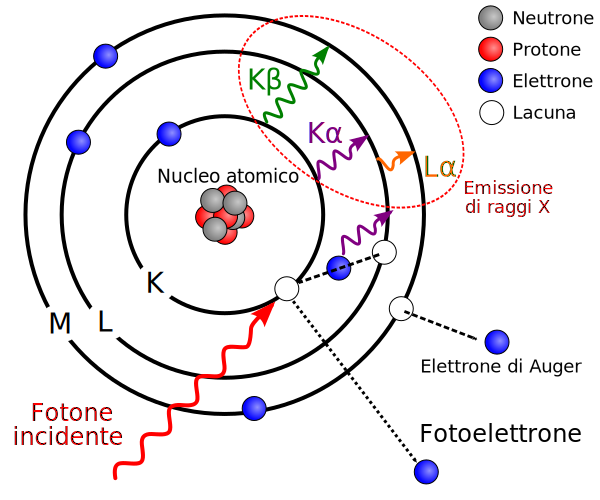
\includegraphics[width=0.9\linewidth]{fotoelettrico.pdf}
		\caption{Schema dell'effetto fotoelettrico e della conseguente emissione di raggi X o elettroni di Auger. Gli orbitali, indicati con notazione spettroscopica M, L e K, producono raggi X con le linee di emissione $K_\alpha$, $K_\beta$ e $L_\alpha$ (cita
			%https://oncologymedicalphysics.com/radiation-interactions/
			).}
		\label{fig:fotoelettrico}
	\end{figure}
	
	\`E possibile ricavare l'andamento approssimativo della sezione d'urto dell'effetto fotoelettrico $\sigma_{fe}$ sia in funzione dell'energia del fotone $E_\gamma$ e del numero atomico $Z$ del bersaglio:
	\begin{equation}
		\sigma_{fe}\propto \frac{Z^4}{E^{\frac{7}{2}}_\gamma}
		\label{eq:sigma_fe1}
	\end{equation}
	sia in funzione dei numeri atomico $Z$ e di massa $A$ del target:
	\begin{equation}
		\sigma_{fe}\propto \frac{Z^5}{A}
		\label{eq:sigma_fe2}
	\end{equation}
	Dalla \hyperref[eq:sigma_fe1]{Eq. 1.28} si osserva che il contributo di $\sigma_{fe}$ diviene particolarmente importante per materiali dotati di atomi pesanti (con alto $Z$) e per basse $E_\gamma$.
	
	\subsubsection{Scattering Compton}
	L'interpretazione corretta dello scattering Compton valse al fisico statunitense Arthur Compton ($1892$--$1962$) il premio Nobel per la fisica nel $1927$.
	
	Nell'esperimento dello scattering Compton proposto dallo stesso scienziato un fascio collimato di fotoni, caratterizzato da una frequenza approssimativamente monocromatica (che corrisponde a una lunghezza d'onda $\lambda_i$), irradia un elettrone appartenente agli orbitali più esterni degli atomi di un blocco di grafite, attuando il processo di diffusione elastica mostrato in \hyperref[fig:compton]{Fig. 1.27}. A differenza dell'\hyperref[par:effetto_fotoelettrico]{effetto fotoelettrico}, si hanno due fotoni prima e dopo l'interazione: il fotone incidente trasferisce quasi tutta la sua energia all'elettrone irradiato mentre il fotone diffuso, a causa del trasferimento di energia all'elettrone, possiede una minore frequenza del primo (che corrisponde a una maggiore lunghezza d'onda $\lambda_f$). Analizzando l'intensità della radiazione diffusa, Compton osservò lo shift in lunghezza d'onda $\Delta \lambda=\lambda_f-\lambda_i$ di raggi X diffusi e incidenti (chiamato Compton shift) e riuscì a spiegare tale fenomeno imponendo la conservazione dell'energia e della quantità di moto dei fotoni e degli elettroni interagenti, ottenendo la \hyperref[eq:compton]{Eq. 1.30}:
	\begin{equation}
		\Delta \lambda=\frac{4\pi\hbar}{m_ec^2}\sin^2{\left(\frac{\theta}{2}\right)}
		\label{eq:compton}
	\end{equation}
	dove $\hbar=\frac{h}{2\pi}$ è la costante di Planck ridotta, $m_e=9.109\cdot^{-31}\mbox{ kg}$ è la massa dell'elettrone (cita
	%https://physics.nist.gov/cgi-bin/cuu/Value?me
	), $c=3.00\cdot10^{8}\mbox{ m/s}$ è la velocità della luce nel vuoto (cita
	%https://physics.nist.gov/cgi-bin/cuu/Value?c|search_for=light
	) e $\theta$ è l'angolo che intercorre tra la direzione del fotone incidente e quella del fotone diffuso.
	
	\begin{figure}[H]
		\centering
		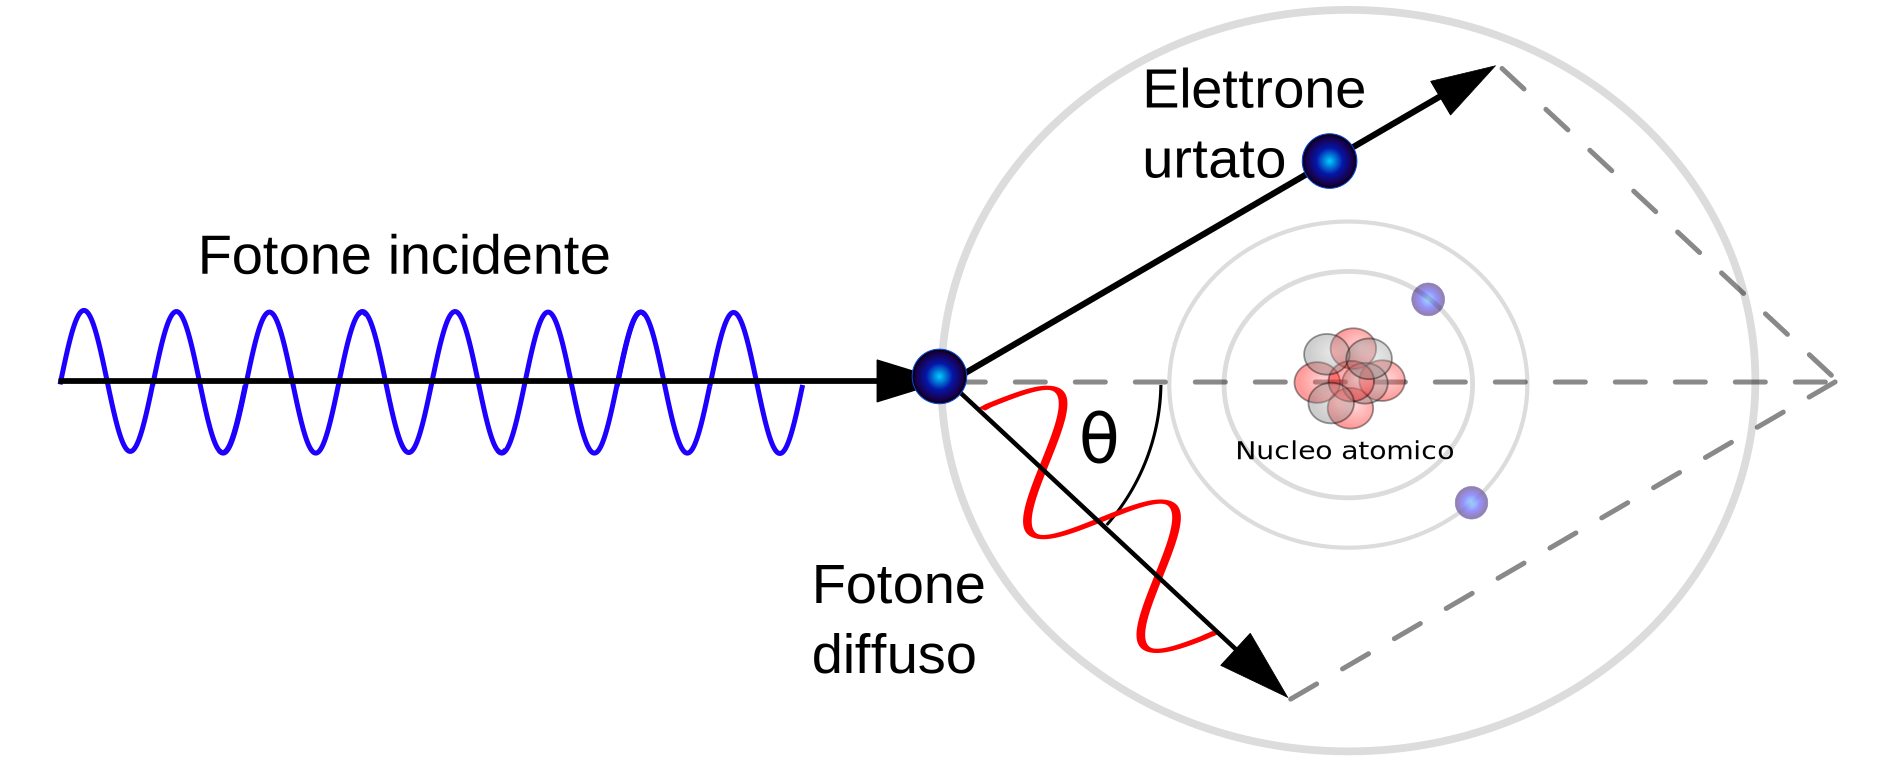
\includegraphics[width=0.9\linewidth]{compton.pdf}
		\caption{Schema dello scattering Compton (cita
			%https://commons.wikimedia.org/wiki/File:Compton_scattering-it.svg
			).}
		\label{fig:compton}
	\end{figure}
	
	\`E possibile ricavare l'andamento approssimativo della sezione d'urto dello scattering Compton $\sigma_{C}$ sia in funzione dell'energia del fotone $E_\gamma$ e del numero atomico $Z$ del bersaglio:
	\begin{equation}
		\sigma_{C}\propto \frac{Z}{E_\gamma}
		\label{eq:sigma_c1}
	\end{equation}
	sia in funzione dei numeri atomico $Z$ e di massa $A$ del target:
	\begin{equation}
		\sigma_{C}\propto \frac{Z}{A}
		\label{eq:sigma_c2}
	\end{equation}
	Dalla \hyperref[eq:sigma_c1]{Eq. 1.31} si osserva che $\sigma_{C}$ viene attenuata linearmente all'aumentare di $E_\gamma$.
	
	\subsubsection{Produzione di coppia}
	La produzione di coppia è un processo di interazione elettromagnetica in cui un fotone, dotato di sufficiente energia ($E_\gamma>2m_e=1.022\mbox{ MeV}$), trasforma tutta la sua energia in massa producendo un elettrone e un positrone secondo il diagramma di Feynman riportato in \hyperref[fig:feynman]{Fig. 1.28}:
	\begin{figure}
		\centering
		\begin{tikzpicture}
			\begin{feynman}[large]
				\vertex (a);
				\vertex [right=of a] (b);
				\vertex [above right=of b] (f1) {$e^-$};
				\vertex [below right=of b] (f2) {$e^+$};
				\diagram* {
					(a) -- [photon, edge label'=$\gamma$] (b) -- [fermion] (f1),
					(b) -- [anti fermion] (f2),
				};
			\end{feynman}
		\end{tikzpicture}
		\caption{Diagramma di Feynman della produzione di coppia elettrone-positrone.}
		\label{fig:feynman}
	\end{figure}
	Non è possibile giustificare tale interazione con le leggi dell'elettromagnetismo classico, ma è necessario il supporto di teorie di campo quantizzato (in questo caso si fa riferimento all'elettrodinamica quantistica o QED) con le quali si può interpretare la trasformazione di energia in materia (e antimateria) che ha luogo durante il processo. La produzione di coppia elettrone-positrone da parte di un fotone avviene solo se quest'ultimo interagisce con un altro corpo (in questo caso o il nucleo atomico o un elettrone, che interagiscono con il fotone per interazione coulombiana; la presenza di un forte campo elettrico è infatti necessaria per consentire la conversione di energia in massa), altrimenti si violerebbe la conservazione del quadrimpulso.\footnote{Nel contesto relativistico la conservazione del quadrimpulso è una generalizzazione della conservazione di energia e quantità di moto.}
	
	Durante la produzione di coppia, l'energia del fotone si ripartisce equamente nell'elettrone e nel positrone ma, successivamente, gli esiti delle due particelle materiali sono differenti: l'elettrone perde energia cinetica generando eventi di ionizzazione mentre il positrone si annichila\footnote{L'annichilazione è il processo inverso alla produzione di coppia in cui un elettrone e un positrone si trasformano in due raggi $\gamma$, convertendo totalmente la loro massa in energia.} con un alto elettrone, producendo due raggi $\gamma$ in direzioni antiparallele (la produzione di un solo raggio $\gamma$ sarebbe impedita dalla conservazione del quadrimpulso) come mostrato in \hyperref[fig:pair_production]{Fig. 1.29}.
	
	\begin{figure}[H]
		\centering
		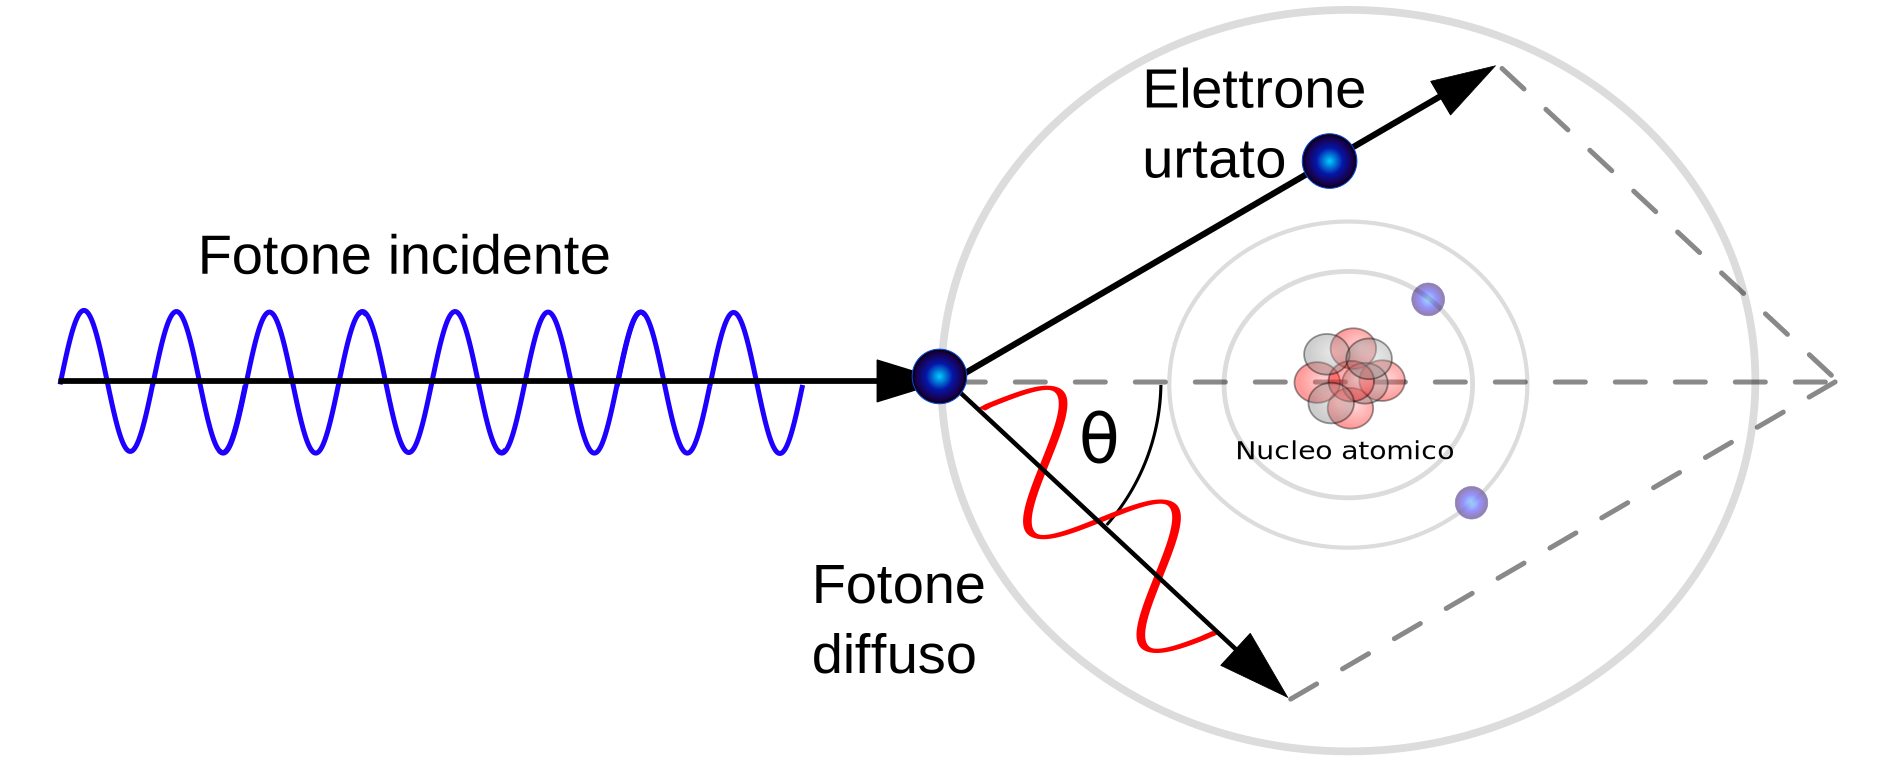
\includegraphics[width=0.9\linewidth]{compton.pdf}
		\caption{Schema della produzione di coppia e successiva annichilazione elettrone-positrone (cita
			%https://upload.wikimedia.org/wikipedia/commons/b/b5/Pairproduction.svg
			).}
		\label{fig:pair_production}
	\end{figure}
	
	Dai diagrammi di Feynman è possibile ricavare l'andamento approssimativo della sezione d'urto della produzione di coppia $\sigma_{pc}$ sia in funzione dell'energia del fotone $E_\gamma$ e del numero atomico $Z$ del bersaglio:
	\begin{equation}
		\sigma_{pc}\propto \frac{Z^2}{\ln{E_\gamma}}
		\label{eq:sigma_pc1}
	\end{equation}
	sia in funzione dei numeri atomico $Z$ e di massa $A$ del target:
	\begin{equation}
		\sigma_{pc}\propto \frac{Z^2}{A}
		\label{eq:sigma_pc2}
	\end{equation}
	Dalla \hyperref[eq:sigma_pc1]{Eq. 1.33} si osserva che $\sigma_{pc}$ è sostanzialmente costante per alte $E_\gamma$.	
	
	La \hyperref[fig:attenuation]{Fig. 1.30} riassume l'andamento della sezione d'urto totale per unità di massa dell'interazione fotone-materia. Si osserva che per basse energie domina l'effetto fotoelettrico, per energie dell'ordine di $1\mbox{ MeV}$ prevale lo scattering Compton e per energie dell'ordine di $10\mbox{ MeV}$ (e maggiori) dominano lo scattering Compton e la produzione di coppia.
	
	\begin{figure}[H]
		\centering
		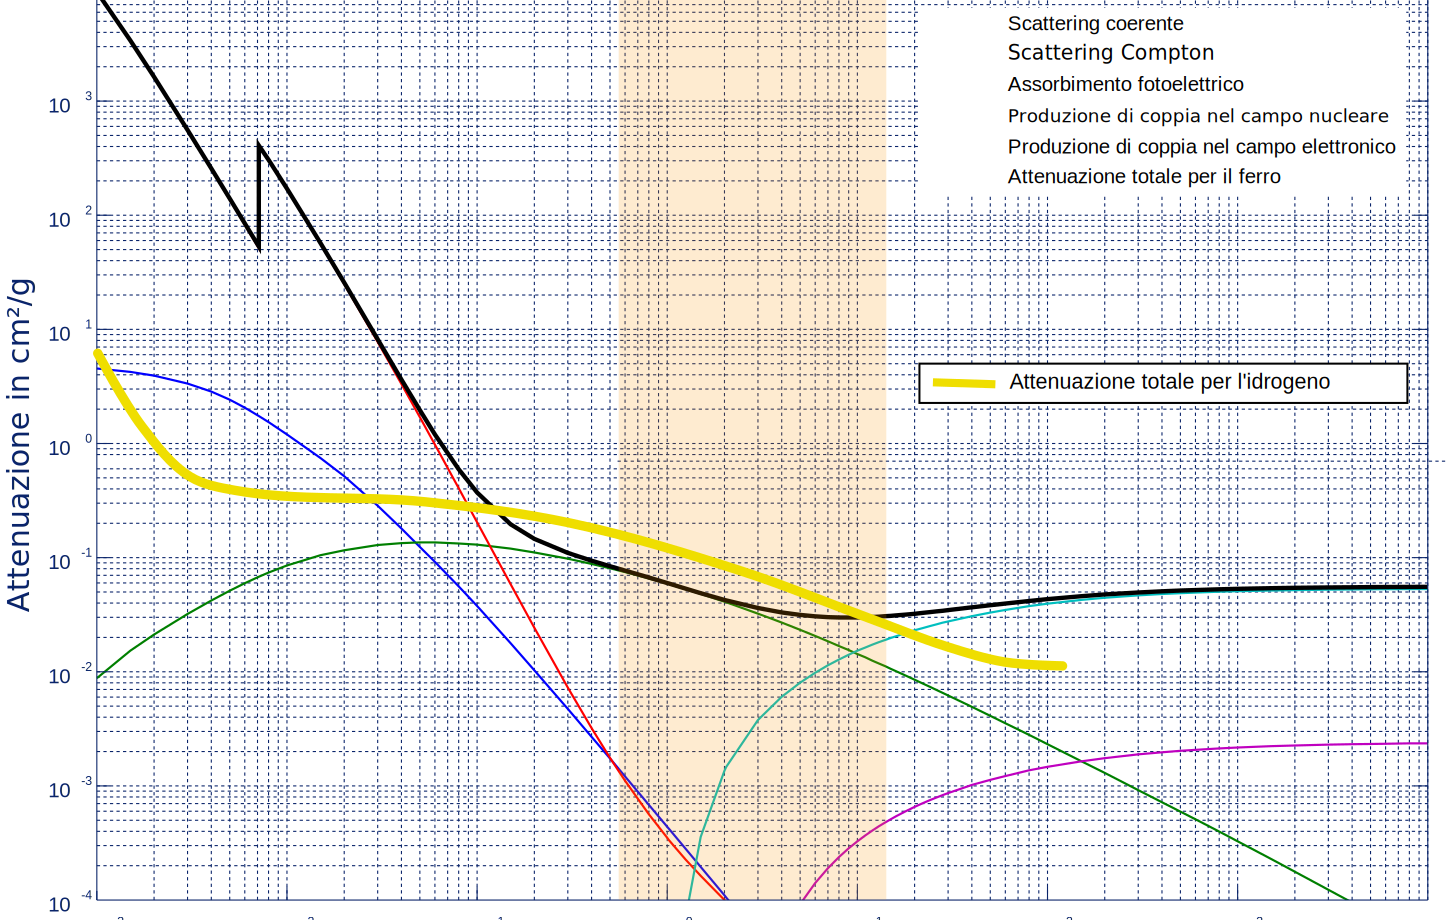
\includegraphics[width=0.9\linewidth]{attenuation.pdf}
		\caption{Andamento della sezione d'urto totale (attenuazione) per unità di massa in funzione dell'energia del fotone incidente in un materiale di ferro e di idrogeno, rappresentati in una scala doppio-logaritmica. Per scattering coerente si intende un tipo di scattering in cui il fotone incidente e quello diffuso possiedono la stessa lunghezza d'onda. Al centro del grafico si evidenzia il range energetico radioterapico (cita
			%https://upload.wikimedia.org/wikipedia/commons/3/3d/Attenuation_Coefficient_Iron-H.svg
			,
			%Maged Marghany, in Nonlinear Ocean Dynamics, 2021
			).}
		\label{fig:attenuation}
	\end{figure}
	
	Essendo il corpo umano principalmente formato da acqua, l'analisi della sezione d'urto totale dell'interazione fotone-acqua risulta essere una buona approssimazione delle interazioni che intercorrono tra i raggi $\gamma$ e il corpo umano durante la radioterapia. Tale situazione viene mostrata in \hyperref[fig:attenuation_water]{Fig. 1.31}, dove è evidente la diminuzione esponenziale della sezione d'urto all'aumentare dell'energia. Ciò avviene perché aumentando l'energia dei raggi $\gamma$ incidenti diminuisce l'attenuazione da parte dell'acqua e quindi si abbassa la probabilità che il fotone interagisca con gli atomi d'acqua e aumenta la sua penetrazione all'interno del bersaglio.

	\begin{figure}[H]
		\centering
		\includegraphics[width=0.9\linewidth]{attenuation_water.png}
		\caption{Andamento della sezione d'urto efficace in funzione dell'energia del fotone incidente in acqua. Si ricorda che il barn (b) è un'unità di misura di superficie tale che $1\mbox{ b}=10^{-24}\mbox{ cm}^{2}$.  (cita
			%https://www.researchgate.net/publication/259002963_Photon_buildup_factors_in_some_dosimetric_materials_for_heterogeneous_radiation_sources
			).}
		\label{fig:attenuation_water}
	\end{figure}
	
	\subsection{Interazione delle particelle cariche con la materia}
	Le particelle cariche interagiscono con la materia in modo più complesso rispetto ai fotoni. Ad esempio, quando le particelle cariche attraversano la materia perdono la loro energia fino ad arrestarsi, un fenomeno che non riguarda i fotoni che quando interagiscono possono essere solamente emessi o assorbiti. Inoltre, le interazioni effettuate dalle particelle cariche sono sia di tipo elettromagnetico che nucleare. In particolare, i processi elettromagnetici sono descritti dalle seguenti interazioni:
	\begin{itemize}
		\item Bethe-Bloch, che avviene con gli elettroni atomici del bersaglio attraverso processi di diffusione anelastici;
		\item scattering Rutherford (o scattering multiplo coulombiano), che avviene con il nucleo del bersaglio attraverso processi di diffusione elastici;
		\item bremsstrahlung (o radiazione di frenamento), che avviene con il nucleo del bersaglio;
		\item effetto Cherenkov, che avviene con gli elettroni atomici e con il nucleo del bersaglio.
	\end{itemize}
	L'interazione elettromagnetica delle particelle cariche con gli elettroni atomici domina sia rispetto alle interazioni nucleari sia rispetto all'interazione elettromagnetica con in nuclei per via delle dimensioni lineari dell'atomo e del suo nucleo. Infatti, essendo l'atomo $10^4$ volte più grande (linearmente) del nucleo, si ha che la sezione d'urto dei processi atomici $\sigma_{atom}$ è più grande di un fattore $10^8$ rispetto alla sezione d'urto che descrive le interazioni nucleari $\sigma_{nucl}$; in particolare, i valori delle sezioni d'urto sono $\sigma_{atom}=100\mbox{ Mb}$ e $\sigma_{nucl}=1\mbox{ b}$. A causa del grande valore di $\sigma_{atom}$ le particelle cariche effettuano moltissime collisioni con gli elettroni atomici, che renderebbe vana una trattazione analitica basata sul calcolo delle sezioni d'urto. Si procede quindi con un approccio energetico in cui si analizza la quantità di energia ceduta dalle particelle cariche durante il loro moto all'interno della materia.
	
	\subsubsection{Bethe-Bloch}\label{par:bethe_bloch}
	Quando una particella carica si muove in un mezzo materiale genera processi di ionizzazione dei suoi atomi dovuti alla forza che esercita sui loro elettroni (cita
	%christoduides libro relatività, capitolo eletromagnetismo
	). Il tasso di energia media persa\footnote{A causa degli eventi di ionizzazione.} per unità di lunghezza lungo il percorso da una particella carica è dato dalla formula relativistica di Bethe-Bloch (o del potere frenante), riportata in \hyperref[eq:bethe_bloch]{Eq. 1.35}:
	\begin{equation}
		\begin{split}
			\left\langle-\frac{dE}{dx} \right\rangle=\frac{\rho Z}{A}\frac{4\pi N_Am_ec^2}{M_U}&\left(\frac{e^2}{4\pi\epsilon_0m_ec^2}\right)^2\cdot\\
			&\cdot\frac{z^2}{\beta^2}\left[\ln{\left(\frac{2m_ec^2\beta^2}{I\left(1-\beta^2\right)}\right)}-\beta^2-\frac{\delta}{2}-\frac{C}{Z}\right]
		\end{split}
		\label{eq:bethe_bloch}
	\end{equation}
	i cui parametri sono riassunti in \hyperref[tab:bethe_bloch]{Tab. 1.3}; si notino sia il segno negativo in $\left\langle-\frac{dE}{dx} \right\rangle$ (che rappresenta perdite di energia) sia l'andamento quadratico rispetto al numero atomico delle particelle del fascio $z$. I processi di interazione descritti dalla Bethe-Bloch sono stocastici: se $n$ particelle identiche aventi tutte la stessa energia iniziale attraversassero un'identica porzione di materiale, in generale subirebbero perdite di energia differenti. La formula di Bethe-Bloch fornisce il valore medio di tali perdite di energia, ma la natura statistica delle stesse ne consente una descrizione più approfondita tramite distribuzioni di probabilità. Ad esempio, se le particelle attraversassero strati sottili di materiali a bassa densità le fluttuazioni delle perdite di energia per unità di lunghezza sarebbero ben descritte da una distribuzione di Landau, altrimenti per spessi strati di materia ad alta densità la distribuzione sarebbe sostanzialmente Gaussiana (a causa del maggiore numero di collisioni che consente l'applicazione del teorema del limite centrale) (cita
	%https://indico.cern.ch/event/387976/attachments/1124401/1605557/daniela_l2.pdf
	,
	%https://it.wikipedia.org/wiki/Formula_di_Bethe
	).
	
	\begin{table}[H]
		\begin{minipage}{\textwidth}
			\centering
			\begin{tabular}{ |M{2cm}||m{12cm}| }
				\hline
				\multicolumn{2}{|c|}{Proprietà del mezzo}\\
				\hline\hline
				$\rho$ & Densità del materiale \\
				\hline
				$Z$ & Numero atomico\\
				\hline
				$A$ & Numero di massa\\
				\hline
				$I$ & Potenziale di ionizzazione\\
				\hline\hline
				\multicolumn{2}{|c|}{Costanti}\\
				\hline\hline
				$N_A$ & Numero di Avogadro\\
				\hline\hline
				$m_e$ & Massa dell'elettrone\\
				\hline
				$M_U$ & Massa molare ($\frac{1}{12}$ della massa di \ce{^{12}C}) \\
				\hline
				$\epsilon_0$ & Costante dielettrica nel vuoto\\
				\hline
				$e$ & Carica dell'elettrone\\
				\hline
				$c$ & Velocità della luce nel vuoto\\
				\hline\hline
				\multicolumn{2}{|c|}{Caratteristiche del fascio}\\
				\hline\hline
				$z$ & Numero atomico delle particelle del fascio\\
				\hline
				$\beta$ & Velocità del fascio in unità di $c$\\
				\hline\hline
				\multicolumn{2}{|c|}{Correzioni}\\
				\hline\hline
				$\delta$ & Correzione di densità, importante ad alte energie\\
				\hline
				$C$ & Correzione di shell, importante a basse energie\\
				\hline
			\end{tabular}
		\end{minipage}
		\caption{Tabella riassuntiva dei parametri della Bethe-Bloch suddivisi in proprietà del mezzo, costanti, caratteristiche del fascio e correzioni. Solitamente si ha $Z/A$$\approx0.42$--$0.5$ e $I\approx19$--$820\mbox{ eV}$.}
		\label{tab:bethe_bloch}
	\end{table}
	
	\`E possibile suddividere l'andamento della Bethe-Bloch (mostrato in \hyperref[fig:bethe_bloch]{Fig. 1.32}) in varie regioni (cita
	%christoduides libro relatività, capitolo eletromagnetismo
	):
	\begin{itemize}
		\item Per energie molto basse l'energia cinetica della particella incidente viene corretta dal fattore $C$ in \hyperref[eq:bethe_bloch]{Eq. 1.35} che include effetti energetici dovuti al moto dell'elettrone attorno al nucleo. In questa regione ci sono anche altre correzioni minori come l'effetto Barkas che tiene conto degli effetti coulombiani causati dalla particella proiettile.
		\item Regione classica: per basse energie ($\beta\gamma<1$)\footnote{$\gamma=1/\sqrt{1-\beta^2}$ è denominato fattore di Lorentz.} il potere frenante diminuisce come $\frac{1}{\beta^2}$ in quanto le particelle cariche più veloci passano meno tempo nelle vicinanze degli atomi della materia, pertanto generano meno processi di ionizzazione.
		\item Regione di minima ionizzazione: per energie più alte ($\beta\gamma\approx3$) si osserva un minimo di ionizzazione dipendente da $\beta$ e (quasi) indipendente dalla massa della particella carica.
		\item Regione relativistica: ad alte energie ($\beta\gamma>4$) si osserva una risalita logaritmica del potere frenante dovuta alla concentrazione delle linee di campo elettrico nella direzione ortogonale alla sua velocità, un effetto puramente relativistico espresso dal termine logaritmico in \hyperref[eq:bethe_bloch]{Eq. 1.35}.
		\item Per energie molto alte la concentrazione delle linee di campo elettrico induce eventi di ionizzazione anche su atomi molto distanti dalla sua traiettoria; ciò induce una polarizzazione negli atomi più distanti che provoca un effetto di schermatura del campo elettrico stesso, inducendo un troncamento nella salita relativistica definito effetto densità. L'effetto di densità è controllato dal fattore $\delta$ in \hyperref[eq:bethe_bloch]{Eq. 1.35}.
	\end{itemize}

	\begin{figure}[H]
		\centering
		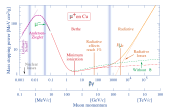
\includegraphics[width=0.9\linewidth]{bethe_bloch.pdf}
		\caption{Valore assoluto del potere frenante per $\mu^+$ in rame in funzione di $\beta\gamma=p/Mc$ dove $p$ è il modulo della quantità di moto relativistica del $\mu^+$. Le bande verticali delimitano varie regioni di approssimazione discusse nel testo. In particolare, la linea verde tratteggiata indicata con $\mu^+$ tiene conto dell'effetto Barkas mentre la linea rossa tratteggiata rappresenta l'azione dell'effetto densità (cita
			%https://pdg.lbl.gov/2022/reviews/rpp2022-rev-passage-particles-matter.pdf
			).}
		\label{fig:bethe_bloch}
	\end{figure}
	
	In \hyperref[fig:adroterapic_range]{Fig. 1.33} viene riportato il potere frenante di un protone per energie molto basse corrispondenti al range utilizzato in adroterapia. Entrambe le \hyperref[fig:bethe_bloch]{Fig. 1.32} e \hyperref[fig:adroterapic_range]{Fig. 1.33} mostrano che il maggior rilascio di energia della particella carica si ha per basse velocità. In altre parole, le particelle cariche rilasciano la quasi totalità della loro energia al termine del loro percorso in uno spazio lineare piuttosto ristretto; è proprio tale peculiarità ha incoraggiato il loro impiego in adroterapia. A tale scopo si definisce il range $R$, ossia la profondità in cui la metà delle particelle cariche penetrate si fermano, definito come:
	\begin{equation}
		R(E_{tot})=\int_{m_0c^2}^{E_{tot}}\frac{dE}{\left(\frac{dE}{dx}\right)}
		\label{eq:range}
	\end{equation}
	dove $m_0$ e $E_{tot}$ sono rispettivamente la massa a riposo e l'energia totale della particella incidente e gli altri parametri sono costanti descritte in \hyperref[tab:bethe_bloch]{Tab. 1.3}. Il range si ottiene integrando il potere frenante fornito dalla \hyperref[eq:bethe_bloch]{Eq. 1.35} su tutto il range energetico rilasciato, calcolo molto complicato vista la complessità della Bethe-Bloch. In generale è possibile approssimare la \hyperref[eq:range]{Eq. 1.36} con una relazione molto utile in adroterapia:
	\begin{equation}
		R(E_{tot})=\alpha E_{tot}^p
		\label{eq:range_approx}
	\end{equation}
	dove $\alpha$ e $p$ sono parametri dipendenti rispettivamente dal bersaglio e dall'energia. Essendo la Bethe-Bloch una legge statistica, le particelle appartenenti a un certo fascio possono potrebbero possedere valori di range caratterizzati da piccole fluttuazioni, conosciute come "range straggling"; ciò risulterebbe problematico in adroterapia nel momento in cui si volessero risparmiare delle regioni tissutali sane nelle vicinanze di un tumore. \`E possibile ricavare che l'incidenza delle fluttuazioni nel range è piuttosto ridotta: ad esempio, irradiando un protone a $200\mbox{ MeV}$ in acqua si ha $R=25.8\mbox{ cm}$ con fluttuazioni di $2.5\mbox{ mm}$ (pari all $1\%$ circa).
	
	\begin{figure}[H]
		\centering
		\includegraphics[width=0.9\linewidth]{adroterapic_range.png}
		\caption{Andamento del potere frenante e del range in funzione dell'energia di un protone in acqua (cita
			%https://www.researchgate.net/figure/Mass-stopping-power-S-versus-ion-energy-E-for-protons-in-liquid-water-The_fig2_274087651
			).}
		\label{fig:adroterapic_range}
	\end{figure}
	
	\subsubsection{Scattering Rutherford, Bremsstrahlung ed effetto Cherenkov}\label{par:scattering_Rutherford}
	Nello scattering Rutherford una particella carica viene deflessa a causa delle interazioni elettromagnetiche multiple indotte dai campi coulombiani dei nuclei del bersaglio. Per via dell'elasticità del processo, ciò che contraddistingue lo scattering Rutherford non è la variazione di energia della particella incidente ma il suo angolo di deflessione a valle dei processi di diffusione multipli, come illustrato in \hyperref[fig:rutherford_scattering]{Fig. 1.34}. Pertanto se l'interazione delle particelle cariche con gli elettroni portava a un range straggling longitudinale\footnote{Per longitudinale si intende parallelo alla direzione del fascio incidente.}, l'interazione delle stesse con i nuclei atomici induce fluttuazioni laterali da considerare nel TP del paziente. Riportando l'esempio dell'irradiazione di un protone a $200\mbox{ MeV}$ in acqua, si hanno fluttuazioni laterali di di $5\mbox{ mm}$ (pari all $2\%$ circa).
	
	\begin{figure}[H]
		\centering
		\includegraphics[width=0.9\linewidth]{rutherford_scattering.pdf}
		\caption{Schema dello scattering Rutherford di una particella carica in un mezzo di spessore $L$ (cita
			%http://www2.ing.unipi.it/~a008137/fis_3_materialedidattico/2017_materiale_didattico/GB-11.1-scattering%20multiplo.pdf
			).}
		\label{fig:rutherford_scattering}
	\end{figure}

	Per determinare la probabilità di interazione per scattering Rutherford si utilizza la sezione d'urto differenziale del processo, riportata in \hyperref[eq:rutherford_scattering]{Eq. 1.38}:
	\begin{equation}
		\frac{d\sigma}{d\Omega}\left(\frac{1}{4\pi\epsilon_0}\frac{Z_1Z_2e^2}{4E_0}\right)^2\frac{1}{\sin^4{\frac{\theta}{2}}}
		\label{eq:rutherford_scattering}
	\end{equation}
	dove $\theta$ è l'angolo di deflessione della particella incidente, $E_0$ è la sua energia, $Z_1$ e $Z_2$ sono rispettivamente il numero atomico della particella e del bersaglio e gli altri parametri sono costanti descritte in \hyperref[tab:bethe_bloch]{Tab. 1.3}.
	
	I contributi apportati dalla Bremsstrahlung ("radiazione di frenamento")\footnote{Nella Bremsstrahlung le particelle cariche decelerano a causa dell'interazione con il campo elettrico coulombiano del nucleo, perdendo energia ed emettendo una distribuzione continua di radiazione (cita
		%note dal corso di fisica biomedica a.a. 2022-2023
		).} e dall'effetto Cherenkov\footnote{Quando una particella carica si muove in un mezzo con una velocità maggiore della velocità della luce in quel mezzo emette radiazione elettromagnetica} risultano trascurabili rispetto alle interazioni descritte nei paragrafi precedenti. In particolare, la Bremsstrahlung risulta trascurabile per le particelle pesanti (come ioni, particelle $\alpha$ e ioni pesanti) in quanto a basse energie $\left(-\frac{dE}{dx}\right)_{Brem}\propto\frac{Z^2}{m^2}$ (dove $Z$ è il numero atomico del target e $m$ è la massa delle particelle proiettile) e l'effetto Cherenkov risulta trascurabile in quanto si verifica per indici di rifrazione del bersaglio $n>0.75$, mentre l'indice di rifrazione del corpo umano (paragonabile a quello dell'acqua) è $n_{acqua}=1.33$.
	
	Riassumendo, le particelle cariche effettuano interazioni elettromagnetiche principalmente con gli atomi elettronici del bersaglio nelle modalità descritte dalla \hyperref[par:bethe_bloch]{Bethe-Bloch} e, in secondo luogo, con i nuclei degli atomi del target tramite \hyperref[par:scattering_Rutherford]{scattering Rutherford}. Come già anticipato nell'analisi della \hyperref[fig:bethe_bloch]{Fig. 1.32}, le particelle cariche perdono la maggior parte della loro energia a bassa velocità, negli istanti di tempo precedenti al loro arresto all'interno del materiale; ciò genera il già citato picco di Bragg, a cui corrisponde un massimo dell'energia rilasciata durante la penetrazione nel bersaglio. Mentre il profilo di dose di particelle cariche pesanti come protoni e ioni carbonio è caratterizzato dal BP, ciò non avviene nel caso dei fotoni (la cui energia viene rilasciata tramite un'attenuazione esponenziale) a causa dei suoi differenti processi di interazione con la materia. Come evidenziato in \hyperref[fig:photon]{Fig. 1.17}, la presenza del BP nel profilo di dose permette un migliore controllo dell'energia depositata nei tessuti del corpo umano, garantendo un'efficienza migliore nella cura dei tumori.
	
	La forte dipendenza della posizione del picco di Bragg dall'energia del fascio incidente (si veda \hyperref[fig:bragg_peak_energies]{Fig. 1.35a}) suggerisce che una corretta scelta di quest'ultima possa far combaciare il volume tumorale presente nel tessuto del paziente con il picco di Bragg, in modo che il maggiore rilascio di dose avvenga nella regione cancerosa. Talvolta la larghezza del BP (pari a $2.5\mbox{ mm}$ per un fascio di protoni a $200\mbox{ MeV}$ in acqua) non è sufficiente a ricoprire l'intero volume tumorale,\footnote{In generale un solo BP non è in grado di ricoprire la struttura tridimensionale di un tumore.} per questo si procede con il SOBP (Spread Out Bragg Peak), tecnica in cui si forniscono più fasci di particelle a diverse energie per generare un picco di Bragg "allargato" (si veda \hyperref[fig:sobp]{Fig. 1.35b}). Chiaramente l'inviluppo degli effetti si ha non solo in corrispondenza della regione tumorale ma anche nel canale di ingresso o subito dopo il BP; nonostante ciò, dalla \hyperref[fig:critical_organ]{Fig. 1.35c} si osserva come l'adroterapia consenta un risparmio maggiore dei tessuti sani rispetto alla radioterapia convenzionale.
		
	\begin{figure}[H]
		\centering
		\begin{subfigure}[t]{0.49\textwidth}
			\centering
			\includegraphics[width=\textwidth, scale=0.50]{bragg_peak_energies.jpg}
			\caption{Andamento del rilascio di dose di fasci protonici in funzione della profondità al variare dell'energia ($60$--$200\mbox{ MeV}$) (cita
				%Literature Review: Characterisation of proton Bragg peak using novel scintillating fibre design for use in proton beam therapy facility (LhARA) Anthea E. MacIntosh-LaRocque Student’s CID: 01507986 Project code: HEPH-Long-1 Supervisor: Prof. Kenneth Long Assessor: Dr. Jaroslaw Pasternak	Word count: 2492
				).}
			\label{fig:bragg_peak_energies}
		\end{subfigure}
		\hfill
		\begin{subfigure}[t]{0.49\textwidth}
			\centering
			\includegraphics[width=\textwidth, scale=0.50]{sobp.pdf}
			\caption{Crazione di SOBP per un fascio singolo di protoni. La curva spessa rappresenta la dose rilasciata nel target (individuato dal cerchio grigio), ottenuta dalla somma dei singoli BP a differenti energie indicati con una linea tratteggiata (cita
				%Walter and Miller's Textbook of Radiotherapy- Radiation Physics Therapy and Oncology
				).}
			\label{fig:sobp}
		\end{subfigure}
		\par
		\begin{subfigure}[t]{0.49\textwidth}
			\centering
			\includegraphics[width=\textwidth, scale=0.50]{critical_organ.jpg}
			\caption{Profili di dose di raggi X, protoni e atomi di carbonio in funzione della profondità. La presenza del BP consente di risparmiare l'organo a rischio, colpito invece dal fascio di raggi X (cita
				%https://fisica.unipv.it/Eventi/Incontri-fisica-moderna/2017-11-28-Tamborini-slides.pdf
				).}
			\label{fig:critical_organ}
		\end{subfigure}
		\caption{Proprietà e applicazioni del picco di Bragg.}
	\end{figure}
	
	Tornando alla \hyperref[fig:photon]{Fig. 1.17} è evidente che il rilascio di energia per il fascio di atomi di carbonio (\ce{C}), a differenza del caso dei protoni (\ce{p}), prosegue anche dopo il BP.\footnote{Un rilascio energetico dopo il BP potrebbe ledere regioni sane situate dopo il volume tumorale, pertanto è necessario comprendere la sua cagione.} Osservando l'andamento quadratico $\propto\frac{z^2}{\beta^2}$ della \hyperref[eq:bethe_bloch]{Eq. 1.35}, pur essendo $z_p<z_C$, si ha che $\frac{dE_p}{dx}>\frac{dE_C}{dx}$ in quanto le energie cinetiche dei carboni sono maggiori di quelle dei protoni.\footnote{Solitamente le energie cinetiche $K$ sono $K_p=250 \mbox{ MeV}$ e $K_C=4800\mbox{ MeV}=12\mbox{ u}\cdot400\mbox{ MeV/u}$.} In effetti il profilo di dose rilasciato dai fasci di $C$ è generalmente maggiore di quello dei $p$ (ciò spiegherebbe i maggiori valori di \hyperref[par:let]{LET} e \hyperref[par:rbe]{RBE} per il carbonio della \hyperref[tab:let_rbe]{Tab. 1.2}), ma ciò non spiega comunque il rilascio di energia dopo il BP. \'E possibile comprendere tale effetto solo analizzando le interazioni nucleari delle due particelle.
	
	\subsubsection{Interazioni nucleari}
	Pur essendo le interazioni elettromagnetiche più frequenti di quelle nucleari, gli effetti di queste ultime risultano fondamentali nelle applicazioni adroterapiche. Per poter effettuare interazioni nucleari con la materia, le particelle cariche devono possedere un'energia sufficientemente elevata da consentire un superamento della barriera di potenziale coulombiana dovuta alle cariche di elettroni e protoni, in modo che i nuclei del proiettile e del bersaglio siano molto vicini tra di loro. Infatti le forze nucleari (come la forza forte che lega i nucleoni\footnote{Protoni e neutroni.} all'interno del nucleo atomico), a differenza della forza elettromagnetica, possiedono una natura a corto raggio d'azione (dell'ordine del raggio dei nucleoni, pari a $\approx1\mbox{ fm}$). Tra i vari effetti delle interazioni nucleari si possono citare il grazing (in cui il nucleo proiettile effettua un "passaggio radente" al nucleo bersaglio generando ad esempio il trasferimento di più nucleoni), collisioni anelastiche (dove i nuclei restano sostanzialmente intatti ma vi è una grande dissipazione di energia) e fusioni nucleari (in cui si genera un nucleo composto che decade dopo $10^{-18}$--$10^{-19}\mbox{ s}$ emettendo raggi $\gamma$, protoni, neutroni, particele $\alpha$ oppure per fissione in frammenti più piccoli) (cita
	%https://www.treccani.it/enciclopedia/reazioni-nucleari-con-ioni-pesanti_%28Enciclopedia-Italiana%29/
	). Nei range energetici utilizzati in adroterapia ($\approx100\mbox{ MeV/u}$) l'interazione nucleare più comune è la frammentazione.
	
	La frammentazione nucleare si suddivide in collisioni periferiche e centrali. Le prime, essendo caratterizzate da bassi scambi di energia e quantità di moto (che avvengono tra i cosiddetti nuclei partecipanti), sono caratterizzate da una bassa molteplicità\footnote{In altre parole generano poche particelle e frammenti del target secondari.}; durante tali eventi si hanno anche nuclei spettatori (sia del proiettile che del target) che si disintegrano mediante processi di frammentazione o evaporazione. Nelle collisioni centrali (meno frequenti delle precedenti) si ha una grande molteplicità di particelle e frammenti generati e vi sono solo nuclei partecipanti, nessun nucleo proiettile (cita
	%https://www.lnf.infn.it/sis/preprint/getfilepdf.php?filename=LNF_81_003(P).pdf
	). La \hyperref[fig:fragmentation]{Fig. 1.36} illustra la dinamica più frequente delle collisioni periferiche suddivisa secondo il modello di Serber (cita
	%Serber, R., 1947, “Nuclear reactions at high energies,” Phys. Rev. 72, 1114–1115.
	) in una fase di abrasione (in cui i nuclei coinvolti interagiscono formando frammenti e uno stato eccitato denominato fireball nucleare) che avviene in tempi di $10^{-22}$--$10^{-23}\mbox{ s}$, e in una di ablazione (dove processi di termalizzazione diseccitano la fireball e producono frammenti secondari sia del proiettile che del bersaglio) che avviene in tempi di $10^{-16}$--$10^{-18}\mbox{ s}$.
	
	\begin{figure}[H]
		\centering
		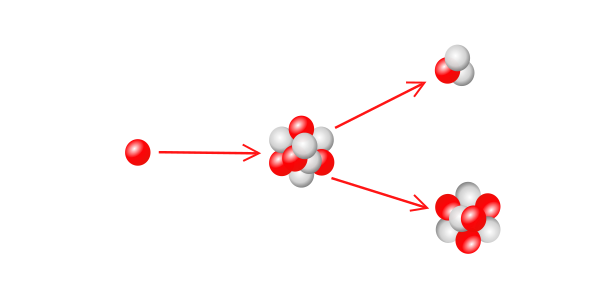
\includegraphics[width=0.9\linewidth]{fragmentation.png}
		\caption{Schema dei processi di abrasione e ablazione (per evaporazione) nel modello di interazione periferica della frammentazione (cita
			%https://www.academia.edu/57450018/Heavy_ion_tumor_therapy_Physical_and_radiobiological_benefits
			).}
		\label{fig:fragmentation}
	\end{figure}
	
	Come già accennato, quando particelle proiettile come \ce{p} o ioni pesanti come \ce{C} colpiscono il corpo umano si può generare una frammentazione sia del proiettile che del target. Sebbene entrambe siano caratterizzati dall'emissione di frammenti leggeri, a seguito della prima si produce anche un quasi-proiettile dotato di un'energia (circa) pari a quella del proiettile incidente mentre a seguito della seconda si genera un quasi-target (circa) a riposo. Le possibilità di frammentazione di un proiettile che interagisce con un target a riposo sono riassunte nella \hyperref[tab:fragmentation]{Tab. 1.4}.
	
	\begin{table}[H]
		\begin{minipage}{\textwidth}
			\centering
			\begin{tabular}{ |M{2.5cm}|M{2.5cm}||m{9cm}| }
				\hline
				Proiettile & Target & Processo\\
				\hline\hline
				Protone & Protone & Non avviene frammentazione\\
				\hline
				Protone & Ione pesante & Frammentazione del target\\
				\hline
				Ione pesante & Protone & Frammentazione del proiettile\\
				\hline
				Ione pesante & Ione pesante & Frammentazione del target e del proiettile\\
				\hline
			\end{tabular}
		\end{minipage}
		\caption{Tabella riassuntiva della frammentazione del target ($\approx200\mbox{ MeV/u}$) e del proiettile (a riposo) in adroterapia per protoni e ioni pesanti.}
		\label{tab:fragmentation}
	\end{table}
	
	 Da un punto di vista pratico è molto complesso studiare i frammenti del target in quanto possiedono un range molto piccolo che va dai $2.3\mbox{ }\mu\mbox{m}$ dell'\ce{^{15}O} al $68.9\mbox{ }\mu\mbox{m}$ dell'\ce{^{2}H} (cita
	 %https://agenda.infn.it/event/11649/attachments/6995/7849/FOOT_Bisogni_220616_PISA.pdf
	 ); in pratica, è come se i frammenti del target venissero prodotti a riposo. Pertanto le proprietà dei frammenti del target non possono essere misurate tramite tecniche di rilevazione convenzionale ma sono necessari approcci differenti come quello della \hyperref[?ref a secondo cap?]{cinematica inversa}, utilizzato nell'esperimento FOOT. D'altra parte, misurare le proprietà dei frammenti del proiettile è più semplice in quanto il loro elevato range consente di applicare metodi di rilevazione convenzionali.
	 
	 Riprendendo la \hyperref[fig:photon]{Fig. 1.17}, ora è possibile comprendere il motivo per cui si verifica un rilascio di dose dopo il BP per particelle cariche pesanti. Tale contributo è dovuto al lungo range dei frammenti del proiettile che, avendo un numero atomico $z$ inferiore al fascio incidente primario, per la \hyperref[eq:bethe_bloch]{Eq. 1.35} possiedono un minore potere frenante;\footnote{Secondo tale considerazione, per penetrare più in profondità basterebbe scegliere fasci formati da particelle con $z$; ciò non è possibile in quanto i processi di frammentazione sarebbero così elevati da rilasciare energie troppo alte nel canale di ingresso, dove si vuole avere un basso dosaggio per risparmiare i tessuti sani. Pertanto ioni più pesanti dell'ossigeno non vengono ritenuti efficaci.} perdendo meno energia per unità di lunghezza i frammenti del proiettile dissipano la loro energia più in profondità rispetto alle particelle proiettile primarie (queste ultime infatti si bloccano generalmente in corrispondenza del picco di Bragg,\footnote{In realtà la sopravvivenza di proiettili primari è fortemente legata alla loro energia e al loro numero atomico (più è grande più interazioni compiono durante il percorso). Ad esempio, un fascio di \ce{^{12}C} a $400\mbox{ MeV}$ ha un range di $28\mbox{ cm}$. A tale profondità il $70\%$ dei \ce{^{12}C} ha già effettuato processi di frammentazione del proiettile prima di giungere al BP; nonostante ciò, nel BP si verifica comunque un grande rilascio di dose generato dalle poche particelle primarie rimanenti e da quelle secondarie.} come mostrato in \hyperref[fig:late_release]{Fig. 1.37}).
	 
	 \begin{figure}[H]
	 	\centering
	 	\includegraphics[width=0.9\linewidth]{late_release.jpg}
	 	\caption{Dati sperimentali della dose totale in funzione della profondità per un fascio di \ce{C} a $400\mbox{ MeV/u}$ in acqua. La diminuzione di energia del fascio primario (curva rossa) nel canale di ingresso è dovuta alla frammentazione che genera frammenti secondari (curva blu) il cui contributo è particolarmente evidente dopo il BP. I due contributi si sommano fornendo la dose totale (curva nera) (cita
	 		%https://indico.cern.ch/event/656460/contributions/2750599/attachments/1685397/2709955/FLUKA_tutorial.pdf
	 		).}
	 	\label{fig:late_release}
	 \end{figure}
	 
	 Dalla \hyperref[fig:biol_effect_nuclear]{Fig. 1.38} è interessante valutare l'effetto delle interazioni nucleari sulle cellule. In particolare si osserva che la frammentazione del target per un fascio di protoni è molto più rilevante nel canale di ingresso che nella regione del picco di Bragg sebbene la ionizzazione nelle due zone sia molto differente. Infatti la ionizzazione uccide rispettivamente il $3\%$ e il $40\%$ delle cellule nel canale di ingresso e nel BP ma l'interazione nucleare è responsabile rispettivamente solo dell'$8\%$ e del $2\%$ delle morti cellulari totali.
	 
	 \begin{figure}[H]
	 	\centering
	 	\includegraphics[width=0.9\linewidth]{biol_effect_nuclear.jpg}
	 	\caption{Impatto dei frammenti di target per un fascio protonico a $250\mbox{ MeV}$ in acqua nel canale di ingresso e nella regione di picco e relativa ionizzazione (cita
	 		%https://www.mdpi.com/2072-6694/7/1/353#
	 		).}
	 	\label{fig:biol_effect_nuclear}
	 \end{figure}
		
	A differenza delle interazioni elettromagnetiche, i processi di frammentazione nucleare non sono solamente più difficili da modellizzare con le teorie di cui disponiamo attualmente, ma anche più complessi da misurare sperimentalmente. Per usufruire delle peculiarità delle particelle cariche (una tra tutte il picco di Bragg) al fine di poter ottimizzare il trattamento clinico dei tumori è necessario giungere a una completa conoscenza dei processi di interazione delle particelle con il corpo umano, in particolare dei processi di frammentazione nucleare, al momento non compresi del tutto. Esistono infatti modelli semiempirici (come la legge di Bradt-Peters) che consentono di ricavare con ottimi risultati le sezioni d'urto di alcune interazioni nucleari conoscendo la struttura dei nuclei del target e del proiettile, ma ciò non è abbastanza: bisognerebbe includere nei modelli la totalità dei contributi forniti dai frammenti nucleari (la cui numerosità è elevatissima). Come verrà esposto nel \hyperref[cap:2]{Cap. 2}, l'obiettivo principale dell'esperimento FOOT (FragmentatiOn Of Target) è proprio quello di arricchire la quantità di dati attualmente a disposizione misurando la sezione d'urto e l'energia di produzione dei frammenti secondari generati a partire dalle interazioni nucleari tra particelle cariche e corpo umano, in modo da migliorare la descrizione di parametri dosimetrici fondamentali nel TP come l'RBE. In particolare, oltre ai fasci di protoni e atomi di carbonio, FOOT intende misurare i frammenti nucleari dei fasci di ossigeno ed elio visto che il loro uso in adroterapia è in fase di sperimentazione.
	
	
	
	
	
	
	
	
	
	
	
	
	%- se vedaimo l'opposto? non la frammentazione del bersaglio, ma la frammentazione del proiettile, ad esempio carbonio contro idrogeno. qui ci sono dei risultati. ma perché quando studio la frammentazione del proiettile ho tuti questi risultati, mentre la frammentazione del bersaglio non c'è niente? il problema è che c'entra la strada che faceva il bersaglio quando veniva frammentato.
	%Ricorda: nel caso di frammentazione del target, avevamo che i frammenti non facevano strada praticamente (pochi micrometri); al contrario, nella frammentazione del proiettile, avevamo che i frammenti percorrono eccome una certa strada.
	%Perché c'entra tutto questo? Immaginiamo di progettare un esperimento di framentazione del bersaglio; abbiamo bisogno di PMNA, ossia targhette del corpo umano con carbonio, idrogeno, ossigeno. qual è lo spessore della targhetta che posso usare? una targhetta sarà di qualche mm, ma sappiamo che nel caso di frammentazione del bersaglio, la strada che fanno i frammenti è di qualche micrometro, per questo i frammenti rimangono bloccati nella targhetta e non è possibile analizzarli: un esperimento "convenzionale" non vedrebbe nulla; allora immaginiamo di ridurre lo spessore della targhetta, per esempio portandolo a qualche micrometro. già un primo problema sarebbe il fatto che con una targhetta così sottile, per avere della buona statistica si dovrebbero aspettare anni, nel senso che gli eventi di diffusione del fascio contro il bersaglio sarebbero pochissimi. Ma mettiamo anche che questo esperimento possa essere fatto, c'è un altro problema: nel momento in cui il frammento fuoriesce dalla targhetta, che è stata fatta molto sottile in modo che i frammenti non rimangano intrappolati nella targhetta stessa, non misuraiamo l'energia di produzione dei frammenti, cioè l'energia che hanno nel momento in cui sono stati prodotti, ma l'energia che hanno dopo che hanno attraversato la targhetta, che sicuramente è un'energia inferiore a quella di produzione visto che dentro la targhetta i frammenti perderebbero energia.
	%Se invece procediamo con la frammentazione del proiettile, questo ha molta energia, oltrepassa la targhetta e li vediamo dai rilevatori, etc.
	%Quindi le tecniche convenzionali funzionano nel caso della frammentazione del proiettile, non funzionano nel caso della frammentazione del bersaglio.
	%
	%- Per questo in FOOT si usano tecniche "non convenzionali". l'idea è che si sfruttano delle trasformazioni di lorentz per "ribaltare" l'esperimento a nostro favore: il bersaglio diventa il proiettile e il proiettile diventa il bersaglio - poi per ripristinare i ruoli in maniera corretta si riapplicano le trasformazioni di lorentz. matematicamenteon è difficile applicare queste trasformazioni, sono matrici sostanzialmente, ma da un punto di vista fisico è difficile, perché ogni trasformazione in più porta con sé delle incertezze maggiori.
	
	
	
	
	
	
%Linear energy transfer is best defined for monoenergetic ions, i.e. protons, alpha particles, and the heavier nuclei called HZE ions found in cosmic rays or produced by particle accelerators. These particles cause frequent direct ionizations within a narrow diameter around a relatively straight track, thus approximating continuous deceleration. As they slow down, the changing particle cross section modifies their LET, generally increasing it to a Bragg peak just before achieving thermal equilibrium with the absorber, i.e., before the end of range. At equilibrium, the incident particle essentially comes to rest or is absorbed, at which point LET is undefined.	
	
% l’idea di usare i protoni per il trattamento del cancro fu proposta per la prima volta nel 1946 L’adroterapia è un forma molto avanzata di radioterapia. La radioterapia, da sola o associata a chirurgia e/o a chemioterapia, migliora il controllo locale in diverse patologie tumorali. Inoltre, la natura non invasiva delle radiazioni rappresenta una valida alternativa per quei tumori non aggredibili chirurgicamente perché localizzati in sedi anatomiche complicate da organi vitali o deputati a funzioni la cui asportazione sarebbe troppo invalidante per il paziente.
	
% La forza dell’adroterapia è nelle proprietà fisiche e radiobiologiche uniche delle particelle cariche (adroni): esse possono penetrare nei tessuti con poca diffusione e depositare la massima energia appena prima di fermarsi. Ciò consente di definire in modo molto preciso la region da irradiare. La caratteristica forma a picco del deposito di energia è chiamata picco di Bragg ed è diventata il simbolo dell’adroterapia.

% dire che FOOT L'esperimento FOOT unisce laboratori giapponesi, tedeschi e italiani al ne di raccogliere dati fondamentali per migliorare la conoscenza delle interazioni tra i fasci adronici e il materiale

% NOTA: end point è il goal che voglio raggiungere. tutti i tumori vicini a organi a rischio hanno percnetuali di soluzione molto molto elevate rispetto alla radioterapia.
	
	
	
	
			
	\addcontentsline{toc}{chapter}{Conclusioni (TBD)}
	\chapter*{Conclusioni (TBD)}
		Let's cite! Einstein's journal paper \cite{einstein} and Dirac's book \cite{dirac} are physics-related items.
	\newpage	
	\printbibliography[
		heading=bibintoc,
		title={Bibliografia}
		]
		 	
\end{document}

